%
% Tesi D.S.I. - modello preso da
% Stanford University PhD thesis style -- modifications to the report style
%
%%%%%%%%%%%%%%%%%%%%%%%%%%%%%%%%%%%%%%%%%%%%%%%%%%%%%%%%%%%%%%%%%%%%%%%%%%%
%                                                                         %
%			TESI DOTTORATO                                                   %
%			______________                                                   %
%                                                                         %
%			AUTORE: Elena Pagani                                             %
%                                                                         %
%			Ultima revisione: 7.X.1998                                       %
%           correzioni atrent                                             %
%%%%%%%%%%%%%%%%%%%%%%%%%%%%%%%%%%%%%%%%%%%%%%%%%%%%%%%%%%%%%%%%%%%%%%%%%%%
%
%
\documentclass[a4paper,11pt]{report}
%    \renewcommand{\baselinestretch}{1.6}      % interline spacing
%
% \includeonly{}
%
%			PREAMBOLO
%
\usepackage[a4paper]{geometry}
\usepackage{amssymb,amsmath,amsthm}
\usepackage{graphicx}
\usepackage{url}
\graphicspath{{./img/}}
\usepackage{hyperref}
\usepackage{epsfig}
\usepackage[italian]{babel}
\usepackage{setspace}
\usepackage{tesi}
\usepackage{enumitem}
\usepackage{float}
\usepackage{parskip}
\usepackage[a-1a]{pdfx}

\usepackage{tabularx}
\usepackage{tcolorbox}
\tcbuselibrary{skins,breakable}

\usepackage{listings}
\usepackage{xcolor}

\lstdefinestyle{azcli}{
    backgroundcolor=\color{yellow!10!white},
    basicstyle=\ttfamily\small,
    frame=single,
    framerule=0.8pt,
    rulecolor=\color{black},
    breaklines=true,
    columns=fullflexible,
    xleftmargin=0pt,
    xrightmargin=0pt,
    aboveskip=8pt,
    belowskip=8pt
}

\usepackage{tcolorbox}
\tcbuselibrary{skins,breakable}

\newtcolorbox{datasetrow}[1]{
    colback=blue!5, colframe=blue!40!black, boxrule=0.6pt, arc=2pt,
    breakable, left=8pt, right=8pt, top=6pt, bottom=6pt,
    title={\textbf{#1}}, fonttitle=\bfseries,
    coltitle=white, colbacktitle=blue!40!black
}


% per le accentate
\usepackage[utf8]{inputenc}
%
\newtheorem{myteor}{Teorema}[section]
%
\newenvironment{teor}{\begin{myteor}\sl}{\end{myteor}}
%
%
%			TITOLO
%
\begin{document}
\begin{center}

\includegraphics[width=\textwidth]{Logo.jpg}
\title{Valutazione della compliance ai CIS Benchmark in ambienti Cloud e on-premise mediante sviluppo di un tool di analisi}
\end{center}
\author{Roberto Antoniello}
\dept{Corso di Laurea magistrale in Informatica} 
\anno{2025-2026}
\matricola{47891A}
\relatore{Prof. Claudio Agostino Ardagna}
\correlatore{Prof. Marco Anisetti}



\beforepreface
\afterpreface
% 
% 
%			CAPITOLO 1: Introduzione
\chapter{Introduzione}

\section{Contesto del problema}

La verifica di conformità alle buone pratiche di un'infrastruttura IT rispetto ad uno standard di sicurezza come i CIS Benchmark richiede il controllo di numerosi parametri di configurazione, ciascuno documentato con criteri specifici. Questo porta al fatto che all'aumentare della dimensione dell'infrastruttura e del numero di controlli di conformità da verificare, l'approccio manuale per questo tipo di lavoro diventa velocemente non sostenibile. \\

Questo tipo di metodo porta quindi con sè dei limiti quali la bassa efficienza in termini di tempo con cui vengono effettuati i controlli e la non scalabilità rispetto all'aumentare delle supervisioni da dover eseguire. Ad esempio se ad un certo punto vi è un aggiornamento dello standard già utilizzato, la conseguenza in tal caso sarebbe rifare nuovamente l'analisi da zero con lo stesso dispendio di tempo.


\section{Obiettivi del lavoro}

Questo progetto si è quindi posto i seguenti obiettivi:
\begin{itemize}
\item Formalizzazione delle buone pratiche di uno standard di sicurezza in forma eseguibile.
\item Quantificazione dell'effort di remediation mediante un modello di scoring
\item Produzione di output dei risultati dell'analisi consultabile per il team operativo.
\end{itemize}

Dunque l'obiettivo è quello di trasformare le raccomandazioni di uno standard di sicurezza in parametri e regole che un tool è in grado di leggere e comprendere in forma automatica senza bisogno di controlli manuali. \\
Non tutti gli oggetti non conformi individuati hanno però lo stesso peso in termini di intervento operativo. Ad esempio alcuni possono richiedere un intervento immediato come la modifica di un semplice parametro di configurazione a impatto zero, mentre altri potrebbero invece richiedere delle attività più complesse che rende necessario un fermo del servizio. \\
Da qui nasce la necessità di introdurre una metrica di effort normalizzata per gli oggetti che risultano non conformi alle buone pratiche. Quindi un valore che rappresenti la complessità, l'impatto sui servizi e la reversibilità di ogni intervento necessario a rendere conformi gli stessi oggetti. \\
Questo porta a poter confrontare gli oggetti e dare un livello di priorità diverso tra i diversi interventi.\\
Quanto detto sopra è chiaramente in funzione del fatto che si riesca ad avere un output finale ben strutturato in modo tale che sia consultabile da chi deve poi andare a eseguire i suddetti interventi. \\

Gli ambienti presi in considerazione durante questo lavoro sono Microsoft Azure per la parte Cloud e VMware per la parte on-premises.

\section{Struttura del lavoro svolto}

Il lavoro svolto in questo progetto è stato eseguito in diverse fasi che verranno descritte in modo più approfondito nei successivi capitoli.\\

Inizialmente vi è stato uno studio dello standard di riferimento che in questo caso è il CIS(Center for Internet Security) Benchmark. I documenti presi in considerazione sono stati i seguenti:
\begin{itemize}
\item CIS Microsoft Azure Foundations Benchmark \cite{CIS_Azure_1}
\item CIS Microsoft Azure Compute Services Benchmark \cite{CIS_Azure_2}
\item CIS VMware ESXi Benchmark \cite{CIS_VMware} \\
\end{itemize}

il CIS Benchmark come standard si presta bene al tipo di lavoro che si pone questo progetto per il fatto che nei documenti CIS i controlli sono descritti e formalizzati in modo tale che per la maggior parte dei controlli descritti vi siano dei criteri di valutazione direttamente traducibili in comandi a livello di codice e quindi automatizzabili mediante lo sviluppo di uno strumento apposito. \\

Da questi documenti sono stati poi estratti un sottoinsieme di controlli di conformità che sono stati implementati nello strumento di analisi. \\
Una volta costruito il dataset, il passo successivo è stato andare a progettare lo schema del framework così da definirne subito i requisiti e il suo funzionamento. \\
Questo ordine di fasi di sviluppo è in funzione del fatto che la progettazione dell'architettura del framework dipende dalla struttura e dal formato del dataset prodotto durante la fase di studio dei documenti CIS e non il viceversa. \\
In questa fase è stato definito anche il modello di scoring rispetto agli interventi di remediation per i controlli che risultano non conformi. \\
Solo successivamente vi è stata la stesura del codice necessario all'implementazione. \\
Infine vi è stata l'analisi dei risultati ottenuti e un resoconto di quanto realizzato.



%			CAPITOLO 2: Standard di riferimento
\chapter{Standard di riferimento e tecnologie utilizzate}

\section{Standard CIS Benchmark}

I benchmark di sicurezza utilizzati in questo progetto sono sviluppati dal CIS(Center for Internet Security).\\
Trattasi di un'organizzazione no-profit riconosciuta a livello globale la cui mission è aiutare le persone, le aziende e i governi delle nazioni a proteggersi meglio dalle vulnerabilità informatiche. \cite{CIS} \\
I sistemi coperti da questa organizzazione sono molteplici, tra i quali anche Microsoft Azure e VMware i cui documenti utilizzati sono stati citati in precedenza.\\ \\ \\

\begin{figure}[h]
	\centering
	
\includegraphics[width=0.6\textwidth]{CIS_logo}
    \caption{Logo del Center for Internet Security (CIS) \cite{CIS}}
    \label{fig:CIS_logo}
\end{figure}



Generalmente i documenti sono un'insieme di buone pratiche che se applicate, vanno a minimizzare il rischio di sicurezza sull'utilizzo dei propri sistemi. Ognuno dei tre documenti utilizzati è suddiviso in diverse sezioni in base alla tipologia di componenti infrastrutturali che vanno a trattare. \\

Di seguito si illustrano i principali campi presenti  nella struttura dei controlli di sicurezza del benchmark: \\
\begin{itemize}
\item \textbf{Titolo}
\item \textbf{Profile Applicability} \\
Diviso tra livello 1 e livello 2. Il primo tratta generalmente le raccomandazioni di sicurezza minima, il secondo invece controlli più approfonditi che potrebbero richiedere attività di riconfigurazione più complesse.
\item \textbf{Description}
\item \textbf{Rationale} \\
Qui vi è una breve descrizione sulla ragione per la quale è rilevante questa raccomandazione di sicurezza.
\item \textbf{Impact} \\
Qui viene descritto l'impatto che la propria infrastruttura può subire nel caso in cui venga adottata la raccomandazione indicata dalla buona pratica CIS.
\item \textbf{Audit} \\
Qui viene descritto come andare a verificare lo stato dell'arte sui propri sistemi per sapere se si è conformi o meno
\item \textbf{Remediation} \\
Qui invece viene descritto come operare per risolvere il problema e risultare conformi.
\item \textbf{Default Value} \\
Qui semplicemente viene indicato qual è il valore di default che detiene la configurazione, spesso quello corretto in termini di sicurezza.
\end{itemize}


Ogni raccomandazione presente all'interno dei documenti CIS riporta inoltra il campo \emph{Assessment Status} che può essere \emph{Automated} oppure \emph{Manual}.
Nel primo caso si tratta di verifiche che possono essere sempre espresse tramite comandi eseguibili in automatico.
Nel secondo caso invece è richiesta dell'interazione manuale come ad esempio la modifica di un impostazione esclusivamente da portale web dell'infrastruttura o la valutazione di una scelta architetturale differente.

Per questo caso di studio la distinzione è rilevante poiché solo le raccomandazioni che possono essere automatizzate rientrano tra quelle candidate per essere tradotte in un sistema automatizzato che valuta la conformità dei controlli.

Di seguito vi è un esempio di un controllo estratto da uno dei documenti dedicati a Microsoft Azure. \\ \\

\begin{tcolorbox}[
    colback=gray!8,
    colframe=gray!40,
    boxrule=0.5pt,
    arc=0pt,
    breakable,
    left=8pt, right=8pt, top=6pt, bottom=6pt
]
\textbf{2.3.4 Ensure 'FTP state' is set to 'FTPS only' or 'Disabled' (Automated)}

\begin{itemize}
    \item \textbf{Profile Applicability:}\\ Level 1
    \item \textbf{Description:}\\ By default, App Service supports deployment over FTP. If FTP is essential for a deployment workflow, FTPS should be enforced for all function apps.
If FTPS is not explicitly required, the recommended setting is \textcolor{red}{Disabled}.
    \item \textbf{Rationale:}\\ FTP is an unencrypted network protocol that transmits data—including passwords—in clear text. The use of this protocol can lead to both data and credential compromise and can present opportunities for exfiltration, persistence, and lateral movement.
    \item \textbf{Impact:} \\
    Deployment workflows that rely on FTP or FTPS rather than WebDeploy or HTTPS endpoints may be affected.\\
	\textbf{Audit}:\\
    \textbf{Audit from Azure Portal}
    \begin{enumerate}
    \item Go to App Services or Function App.
    \item Click the name of a function app.
    \item Under Settings, click Configuration.
    \item In the General settings pane, under Platform settings, ensure that FTP state is set to FTPS only or Disabled.
    \item Repeat steps 1-4 for each function app.
    \end{enumerate}
	\textbf{Audit from Azure CLI} \\
	Run the following command to list function apps: \\
	
	\begin{lstlisting}[style=azcli]
	az functionapp list
	\end{lstlisting}


For each function app, run the following command to get the FTPS state setting:
	\begin{lstlisting}[style=azcli]
	az functionapp show --resource-group <resource-group-name> --name <function-app-name> --query siteConfig.ftpsState
	\end{lstlisting}
Ensure that \textcolor{red}{"FtpsOnly"} or \textcolor{red}{"Disabled"} is returned.
\end{itemize}
\end{tcolorbox}



Nell'esempio mostrato si evidenziano due aspetti ricorrenti nei controlli all'interno del benchmark Azure.
L'audit è descritto sia tramite portale web sia tramite Azure CLI e la verifica deve essere chiaramente ripetuta per ogni risorse del tipo coinvolto.\\
Per quanto riguarda i documenti VMware la struttura è la medesima, con la differenza che le modalità di verifica spaziano tra il vSphere CLient, PowerCLI ed ESXCLI.

I test eseguiti durante lo svolgimento del lavoro si sono limitati a tutti quei controlli compatibili con la sottoscrizione Azure a disposizione: Azure For Student. \\
Per quanto riguarda invece VMware è stato possibile utilizzare ai fini del progetto un'infrastruttura di laboratorio aziendale presso Lutech S.p.A.


\subsection{Perimetro dei documenti CIS utilizzati}

La seguente tabella~\ref{tab:benchmark} riassume in breve quanti controlli sono stati estratti per l'implementazione tra i tre documenti utilizzati in fase di studio del benchmark.

\begin{table}[H]
\centering
\small
\begin{tabular}{llrrrr}
\hline
\textbf{Documento} & \textbf{Versione} & \textbf{Raccomandazioni} &
\textbf{Automated} & \textbf{Manual} & \textbf{Implementate} \\
\hline
Azure Foundations     & 5.0.0 & 155 & 93 & 62 & 39 \\
Azure Compute Services & 2.0.0 &  99 & 77 & 22 & 21 \\
VMware ESXi 8         & 1.2.0 & 134 & 38 & 96 & 39 \\
\hline
\end{tabular}
\caption{Documenti CIS utilizzati e raccomandazioni implementate}
\label{tab:benchmark}
\end{table}


Nell'insieme di buone pratiche implementate per VMware vi è anche un controllo classificato come \emph{Manual}, per il quale è stato comunque possibile definire una verifica da PowerCLI sulla configurazione della macchina virtuale.

I due documenti del benchmark CIS di Azure coprono ambiti diversi.
Foundations si occupa principalmente delle impostazioni della sottoscrizione attiva e dei servizi di base.\\
Compute Services invece si dedica ad altre macroaree come le App Service e le virtual machines.
Su VMware nell'unico documento utilizzato si ha che le raccomandazioni sono distribuite sotto 8 sezioni, spaziando dall'hardware fisico alla configurazione delle virtual machines.

Il perimetro di questo progetto è limitato quindi a un sottoinsieme di questi documenti.\\
Le seguenti tabelle~\ref{tab:sez-az} e~\ref{tab:sez-vmw} illustrano, per ogni sezione coperta, quante buone pratiche contiene e quante di queste sono state implementate nello strumento di analisi sviluppato.\\
I dettagli implementativi sono rimandati nel capitolo 4.

\begin{table}[H]
\centering
\small
\begin{tabular}{llrr}
\hline
\textbf{Sezione} & \textbf{Documento} & \textbf{Totale} & \textbf{Implementate} \\
\hline
6 - Logging and Monitoring & Foundations & 25 & 15 \\
7 - Networking Services    & Foundations & 16 & 11 \\
8 - Security Services      & Foundations & 38 & 13 \\
2 - App Service            & Compute     & 77 & 15 \\
20 - Virtual Machines      & Compute     & 11 &  6 \\
\hline
\end{tabular}
\caption{Copertura del benchmark Azure per sezione}
\label{tab:sez-az}
\end{table}

\begin{table}[H]
\centering
\small
\begin{tabular}{lrr}
\hline
\textbf{Sezione} & \textbf{Totale} & \textbf{Implementate} \\
\hline
2 - Base             & 12 &  3 \\
3 - Management       & 26 & 10 \\
4 - Logging          & 11 &  1 \\
5 - Network          & 11 &  5 \\
6 - Features         & 18 &  1 \\
7 - Virtual Machines & 29 & 19 \\
\hline
\end{tabular}
\caption{Copertura del benchmark VMware per sezione}
\label{tab:sez-vmw}
\end{table}


\section{Tecnologie}

Data la natura degli ambienti e della struttura dei benchmark, il linguaggio di programmazione scelto è stato PowerShell. \\
Questo linguaggio è risultato il più funzionale rispetto a questo lavoro poiché all'interno dei documenti CIS tutti gli automatismi di audit e di remediation sono scritti in PowerShell. \\
Dunque non vi è stato necessario adattare i comandi per farli eseguire da un'altra tecnologia, ma sono stati utilizzati i suggerimenti ufficiali dettati dal Center for Internet Security. \\ \\
Per quanto riguarda Azure la componente principale è Azure CLI, utilizzata per interagire con l'infrastruttura cloud.\\
Per quanto riguarda VMware viene utilizzato il modulo VMware PowerCLI per interrogare il vCenter.

%			CAPITOLO 3: Architettura framework
\chapter{Architettura del framework}


\section{Schema architetturale del tool}

In questo paragrafo ci soffermiamo brevemente su come è stato progettato il flusso delle operazioni svolte dal tool di analisi. \\

Gli schemi concettuali mostrati di seguito sono speculari per quanto riguarda Azure e VMware, differendo sostanzialmente nelle rispettive sezioni dei documenti CIS coperte.\\
L'esecuzione è stata strutturata in tre fasi diverse:
\begin{itemize}
\item \textbf{Connessione infrastruttura.} \\
L'utente si autentica su Azure o VMware collegandosi alla propria infrastruttura di riferimento sulla quale vuole eseguire l'analisi di conformità ai CIS benchmark.
\item \textbf{Esecuzione.} \\
Sequenzialmente avviene l'analisi sezione dopo sezione mostrando in tempo reale la conformità o non dei controlli eseguiti. Allo stesso tempo, i risultati dei test vengono salvati in memoria per la terza e ultima fase.
\item \textbf{Export report.} \\
Una volta completati tutti i controlli, il software va a riepilogare a schermo i risultati e successivamente li esporta in un file di report in formato .csv. Da qui comincia la consultazione per il team operativo. \\\\\\\\\\\\\\\\\\\\
\end{itemize}



\begin{figure}[h]
	\centering
	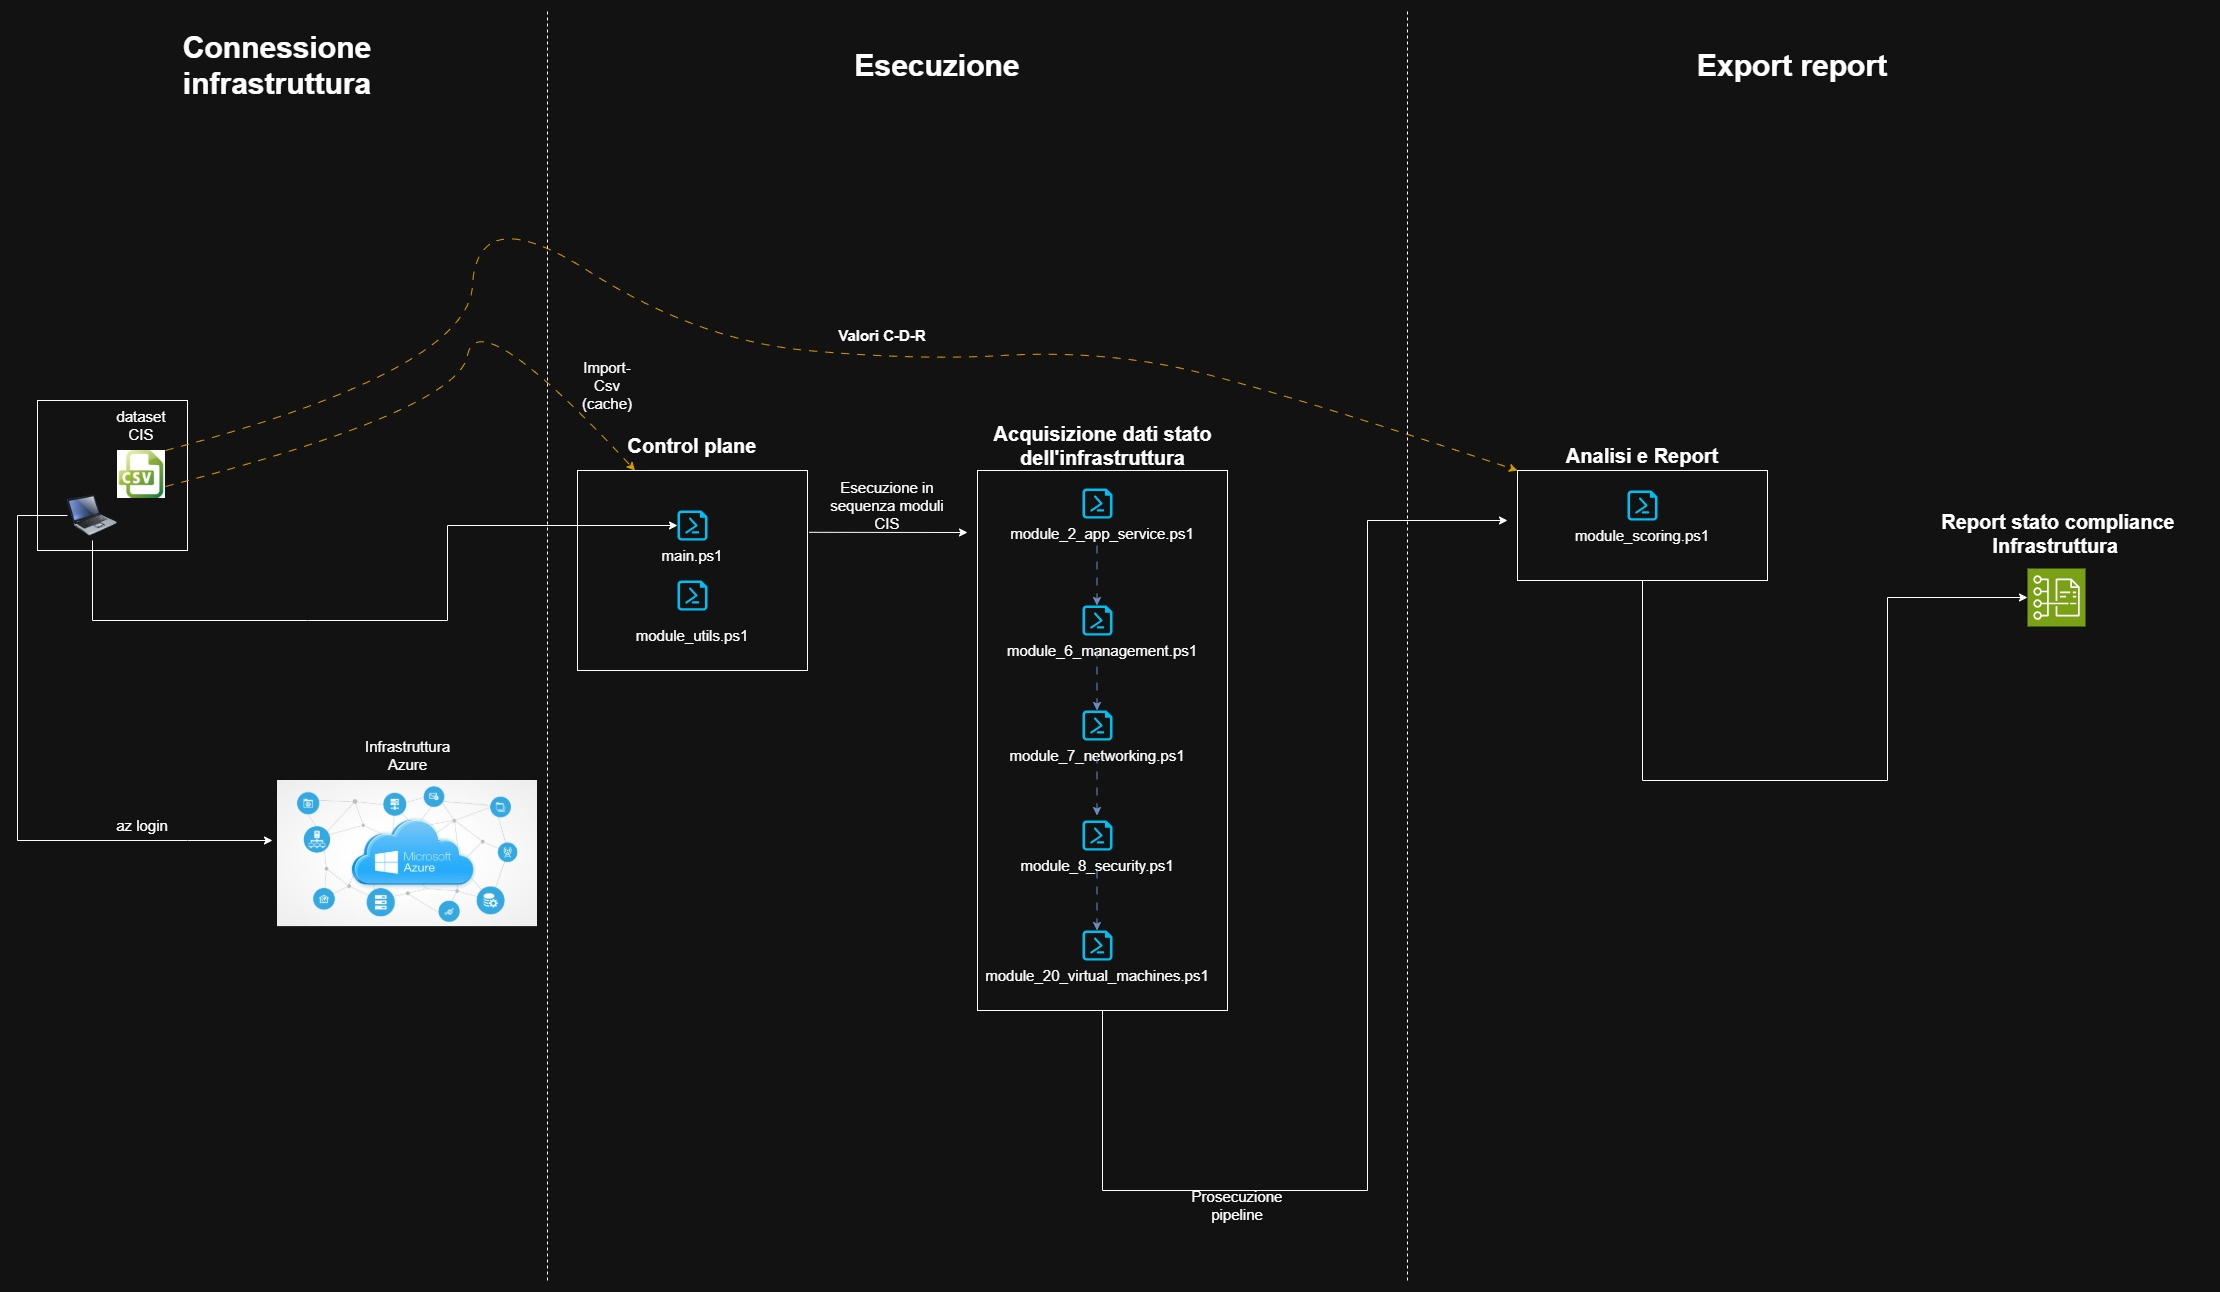
\includegraphics[width=1.0\textwidth]{architettura_script_cis_Azure}
    \caption{Schema concettuale della funzionalità per Azure}
    \label{fig:architettura_script_cis_Azure}
\end{figure}

\begin{figure}[h]
	\centering
	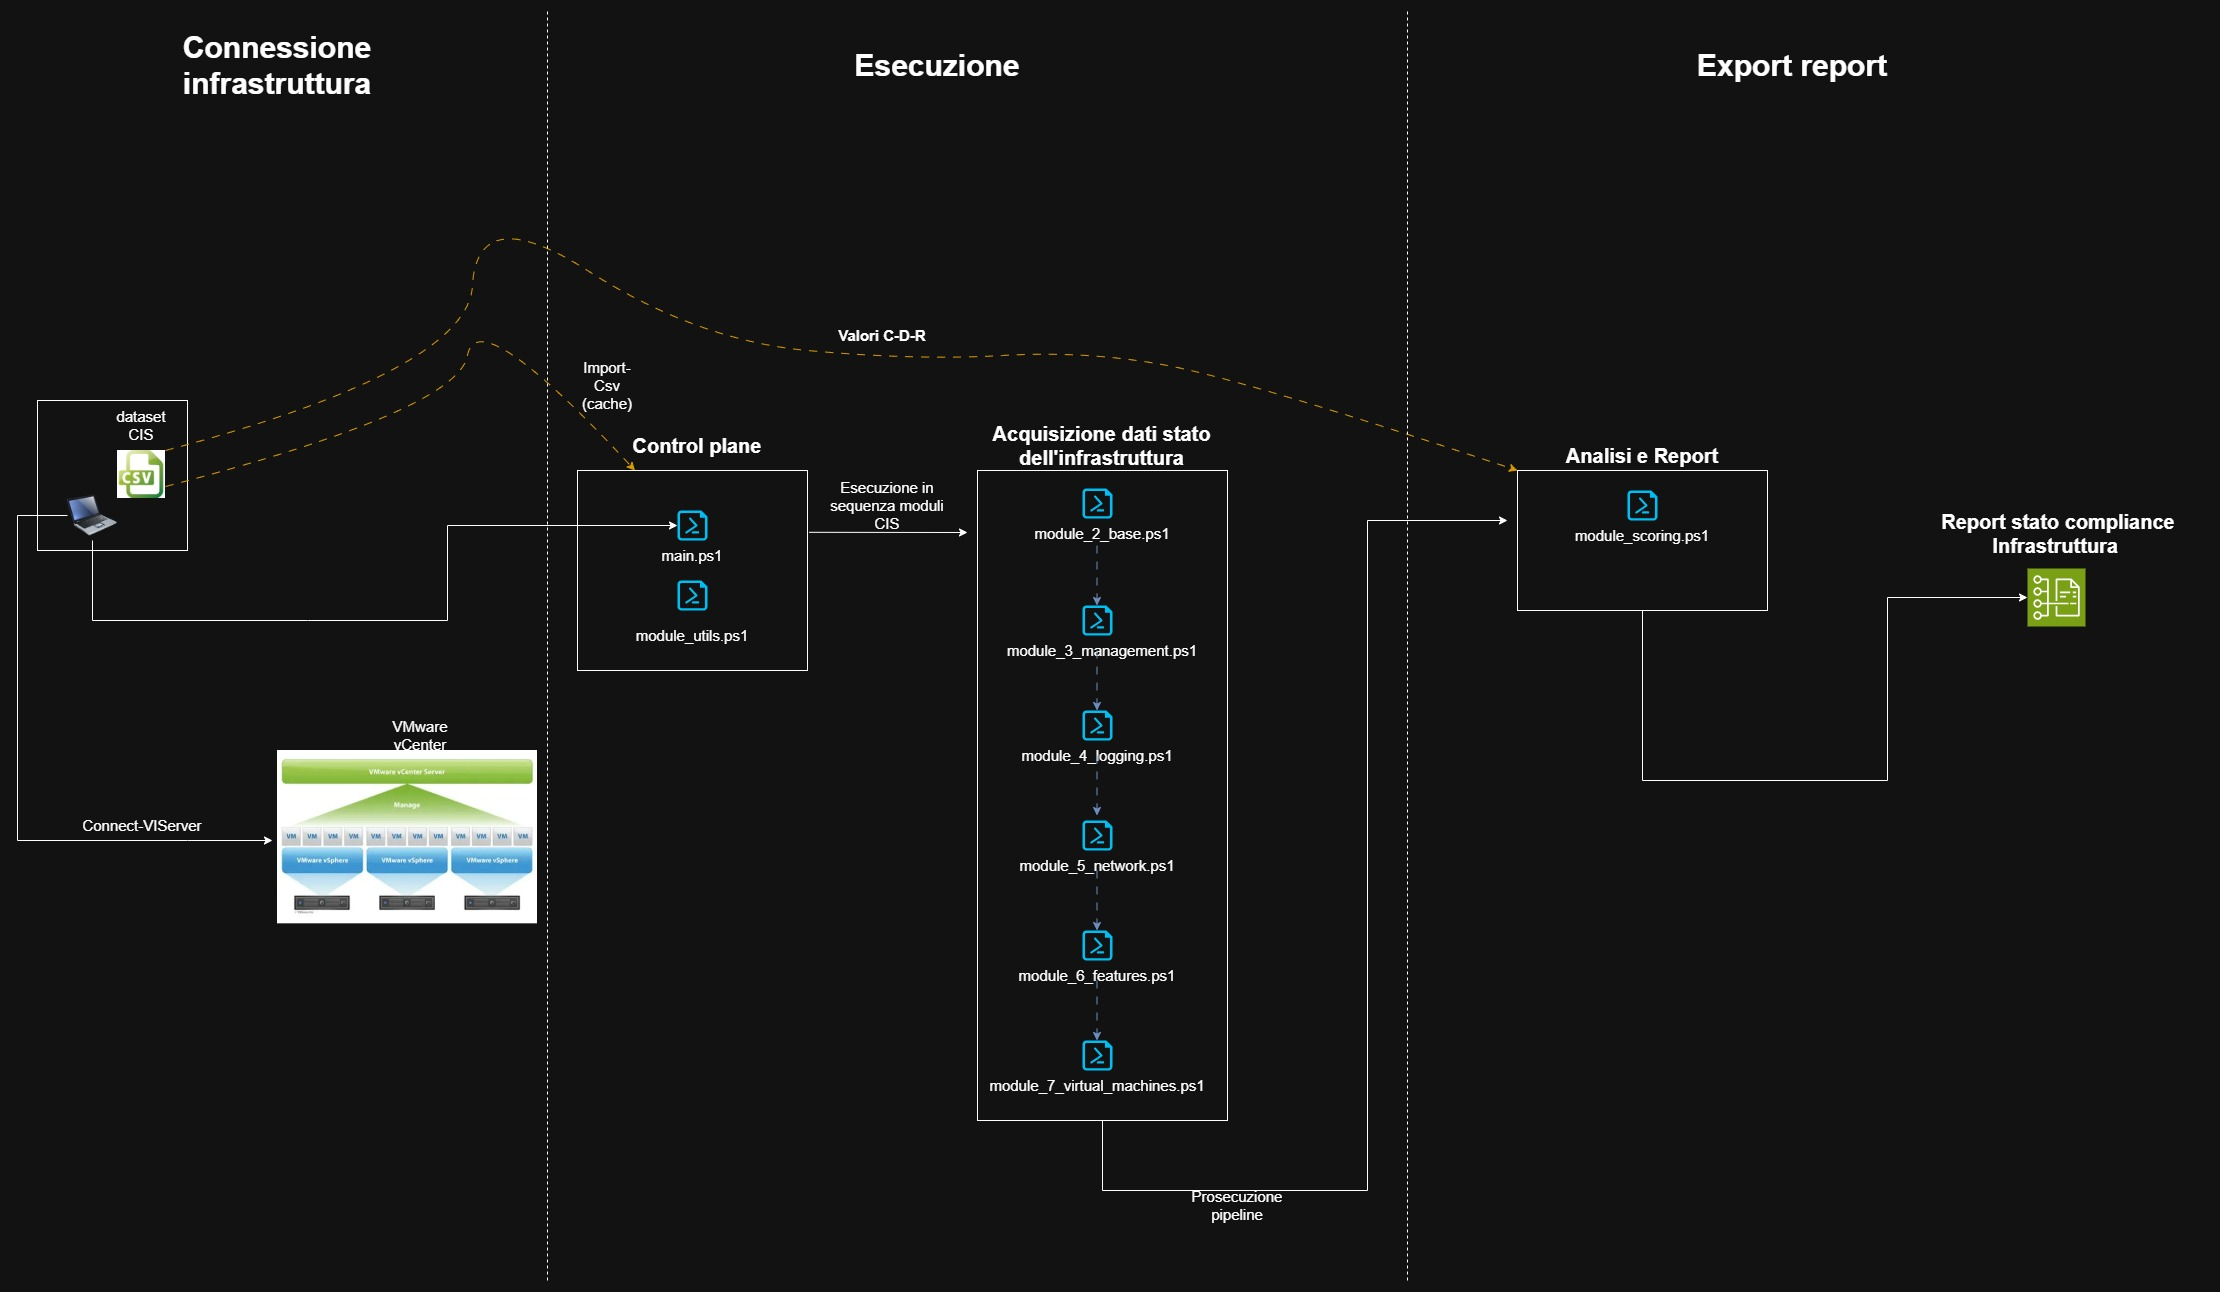
\includegraphics[width=1.0\textwidth]{architettura_script_cis_VMware}
    \caption{Schema concettuale della funzionalità per VMware}
    \label{fig:architettura_script_cis_Azure}
\end{figure}



\section{Dataset estratto dai documenti CIS Benchmark}

La costruzione del dataset è stata fondamentale per riuscire ad avere un input strutturato da poter sottoporre al framework. \\
L'estrazione del sottoinsieme di controlli è avvenuto andando a verificare ciò che poteva essere rilevante mostrare come test dimostrativo, oltre a escludere ciò di cui non era possibile computare l'analisi a causa della sottoscrizione \textit{Azure for Student}. \\

Ogni riga del dataset è composta dalla maggior parte dei campi di un controllo CIS, già citati nel capitolo precedente. \\
In aggiunta a questi, vi sono i seguenti attributi:
\begin{itemize}
 \item C
 \item D
 \item R
 \item setting-name
 \item expected-value
 \item operator 
 \end{itemize} 
 
 I primi 3 riguardano la complessità, indisponibilità e reversibilità rispetto all'eventuale intervento di remediation degli oggetti non conformi. Verranno approfonditi nel capitolo 5 dedicato al modello di scoring ideato e utilizzato. \\
Gli altri tre attributi riguardano invece rispettivamente il nome del parametro di configurazione, il suo valore atteso e l'operatore di comparazione che verranno utilizzati per verificare la conformità. \\
In questo modo tutti quei controlli che sono standardizzabili, forniranno i dati per il controllo direttamente dal dataset. \\
Tutto ciò che sfortunatamente non è possibile standardizzare, avrà il valore \textit{"custom"} sull'attributo operator e una funzione dedicata nel sorgente. \\

Qui di seguito un esempio di una riga estratta dal dataset per Azure e VMware in formato scheda per leggibilità. \\

\begin{datasetrow}{(Azure)2.3.3 --- Ensure 'Basic Authentication Publishing Credentials' are 'Disabled'}

\begin{description}
    \item[Category] app-service
    \item[Profile Applicability] Level 1
    \item[Description] Basic Authentication Publishing Credentials provides the ability to publish---or deploy to---a function app without a centralized Identity Provider. For a more effective, capable, and secure solution for Identity, Authentication, Authorization, and Accountability, a centralized Identity Provider such as Entra ID is strongly advised.
    \item[Rationale] Basic Authentication introduces an identity silo for privileged access to a resource and produces logging which may not provide a full chain of accountability. This can be exploited in numerous ways and represents a significant vulnerability and attack vector.
    \item[Impact] Disabling 'Basic Auth Publishing Credentials' will prevent the following deployment methods from working: FTP $\cdot$ FTPS $\cdot$ FTPS SCM Basic Auth Publishing Credentials $\cdot$ Local Git $\cdot$ GitHub $\cdot$ Azure Repos $\cdot$ Bitbucket $\cdot$ Visual Studio (Version 17.12 and earlier). If this recommendation cannot be implemented because one of the above listed deployment methods is necessary and cannot be adapted, compensating controls (e.g. using FTPS only and disabling only "SCM Basic Auth Publishing Credentials") are recommended to reduce potential attack surface.
\end{description}
\vspace{2pt}
\noindent\textbf{Audit:}
\begin{lstlisting}[style=azcli]
    az functionapp list
    az resource show --resource-group <resource-group-name> --name <function-app-name> --resource-type "Microsoft.Web/sites" --query basicPublishingCredentialsPolicies
\end{lstlisting}

\noindent\textbf{Remediation:}
\begin{lstlisting}[style=azcli]
az resource update --resource-group <resource-group-name> --name <function-app-name> --resource-type "Microsoft.Web/sites" --set properties.allow=false
\end{lstlisting}

\vspace{4pt}
\noindent
\textbf{C} = 1 \quad
\textbf{D} = 0 \quad
\textbf{R} = 1 \quad
\textbf{setting-name} = \texttt{properties.allow} \quad
\textbf{expected-value} = \texttt{false} \quad
\textbf{operator} = \texttt{custom}

\end{datasetrow}




\begin{datasetrow}{(VMware)2.4 --- Host image profile acceptance level must be 'PartnerSupported' or higher}

\begin{description}
    \item[Category] base
    \item[Profile Applicability] Level 1
    \item[Description] The acceptance level on ESXi regulates the type of software that can be installed on the system, with four distinct levels: VMwareCertified, VMwareAccepted, PartnerSupported, and CommunitySupported. It's advised to set the acceptance level to PartnerSupported or higher to ensure that only tested and digitally signed vSphere Installation Bundles (VIBs) are allowed for installation.
    \item[Rationale] The ESXi Image Profile should only allow signed VIBs because an unsigned VIB represents untested code installed on an ESXi host. Also, use of unsigned VIBs will cause hypervisor Secure Boot to fail to configure. Community Supported VIBs do not have digital signatures. To protect the security and integrity of your ESXi hosts, do not allow unsigned (CommunitySupported) VIBs to be installed on your hosts.
    \item[Impact] Restricting the acceptance level to PartnerSupported or higher prevents the installation of CommunitySupported packages, which are unsigned and hence, potentially unreliable or insecure. This restriction, while enhancing security, might limit the range of software that can be installed on the ESXi host
\end{description}

\vspace{2pt}
\noindent\textbf{Audit:}
\begin{lstlisting}[style=azcli]
# List only the vibs which are not at "VMwareCertified" or
# "VMwareAccepted" acceptance level
Foreach ($ESXCli in Get-VMHost | Get-EsxCli -VMHost $VMHost) {
    $ESXCli.software.acceptance.Get("PartnerSupported")
}
\end{lstlisting}

\noindent\textbf{Remediation:}
\begin{lstlisting}[style=azcli]
# Set the Software AcceptanceLevel for each host
Foreach ($ESXHost in Get-VMHost) {
    $ESXCli = Get-EsxCli -VMHost $ESXHost
    $ESXCli.software.acceptance.Set("PartnerSupported")
}
\end{lstlisting}

\vspace{4pt}
\noindent
\textbf{C} = 1 \quad
\textbf{D} = 0 \quad
\textbf{R} = 1 \quad
\textbf{setting-name} = \texttt{VMwareCertified | VMwareAccepted | PartnerSupported} \quad
\textbf{expected-value} = --- \quad
\textbf{operator} = \texttt{custom}

\end{datasetrow}


\section{Requisiti e gestione del flusso}

I requisiti di esecuzione sono chiaramente diversi tra i due ambienti trattati e sono i seguenti. \\
Su Microsoft Azure è necessario essere in possesso di una sottoscrizione valida ai fini dell'autenticazione mediante il comando \textit{"az login"}. \\
Per VMware invece è necessario essere in possesso delle credenziali di amministratore per potersi autenticare su un vCenter mediante il comando \textit{"Connect-VIServer"}.\\

È possibile parametrizzare il lancio del framework come ad esempio aggiungere il flag che permette di salvare come log in un file di testo ogni output del terminale. Sempre da linea di comando è possibile la personalizzazione dei pesi dei già citati parametri C, D, R che verranno poi approfonditi in seguito. \\


Le uniche differenze nel flusso di esecuzione tra Azure e VMware riguardano l'inizializzazione del programma, il quale andrà a caricare in memoria il rispettivo dataset. Fatto questo viene chiamato il relativo main in funzione dell'ambiente e come detto in precedenza, vengono eseguiti sequenzialmente i controlli.


\section{Struttura interna del tool}

Finora è stato descritto il framework ad alto livello dal punto di vista di chi lo utilizza, quindi le fasi di esecuzione, i requisiti e il formato del dataset.\\
A questo punto si va più in profondità ad analizzare le componenti che compongono lo strumento, le interazioni e il percorso che un singolo controllo segue dall'inizio alla fine.


\subsection{Componenti e dati condivisi}

Il seguente diagramma mostra le componenti del framework e il flusso di lettura/scrittura dei dati durante l'esecuzione.


\begin{figure}[H]
	\centering
	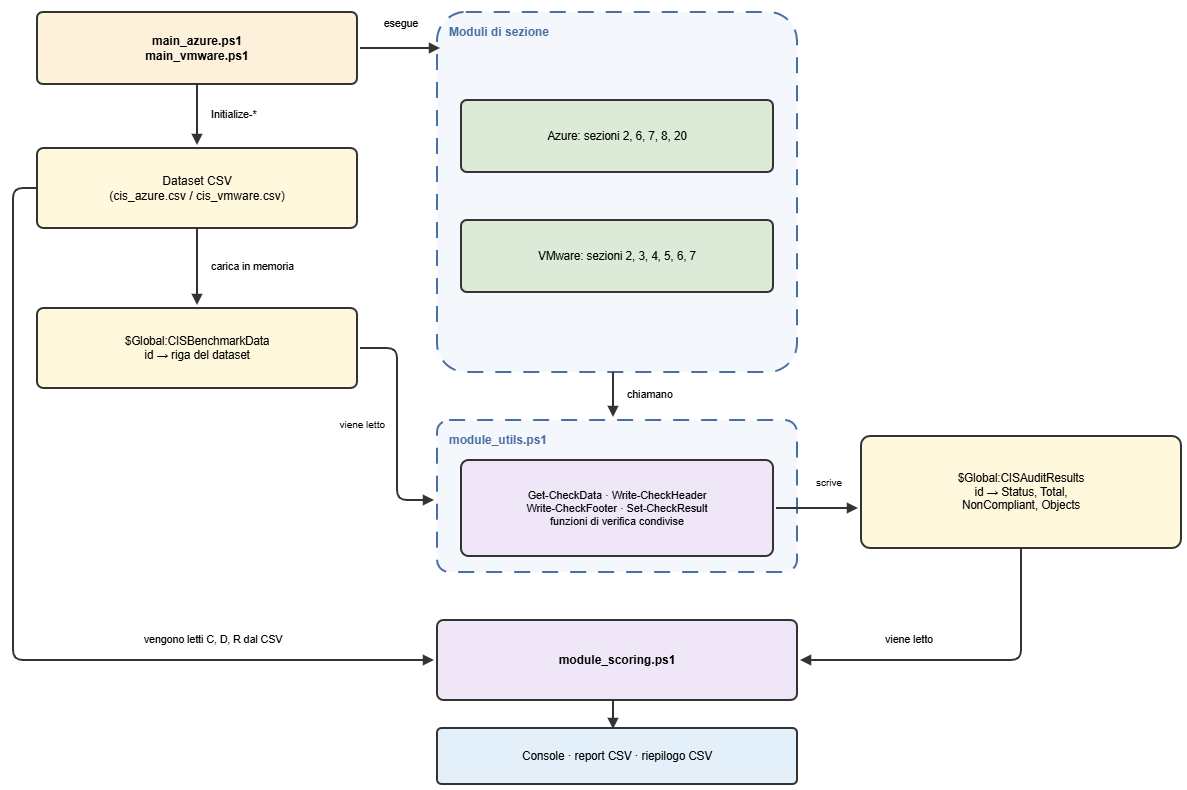
\includegraphics[width=\textwidth]{architettura_componenti}
	\caption{Diagramma strutturale a basso livello del tool sviluppato.}
	\label{fig:componenti}
\end{figure}

Come è possibile osservare il punto di ingresso iniziale è il main dell'ambiente che si intende analizzare.
Come prima operazione viene richiamata una funzione di inizializzazione che procede a verificare l'esistenza di una sessione autenticata sull'infrastruttura da valutare e infine carica in memoria il dataset, il quale è indicizzato dall'identificativo del controllo CIS.

Da questo momento, qualsiasi funzione può recuperare i dati di un controllo(nome, parametro da interrogare, valore atteso, operatore di confronto, remediation) a partire dall'identificativo come chiave. \\
La stessa funzione di inizializzazione si occupa inoltre di creare un registro dei risultati, un'altra struttura chiave-valore inzialmente vuota all'interno della quale verranno man mano registrati gli esiti dei controlli effettuati.

In un secondo momento, il main esegue in sequenza i moduli delle varie sezioni previste implementate. L'unica componente condivisa tra i moduli e il main è il sorgente \texttt{module\_utils}, il quale contiene funzioni di sistema come ad esempio le operazioni descritte poco fa e funzioni ausiliarie per rendere la logica di verifica dei controlli nei moduli meno complessa.\\
Al termine dell'esecuzione di ogni controllo, come già anticipato, viene scritto l'esito nel registro dei risultati che per ogni identificativo salva quattro campi di informazione.

\begin{itemize}
	\item Lo stato del controllo(conforme/non conforme).
	\item Il numero totale di oggetti valutati.
	\item Il numero di oggetti non conformi.
	\item Il dettaglio degli oggetti non conformi, che viene poi mostrato nel report finale.
\end{itemize}

il modulo dedicato allo scoring è l'unica componente che va ad utilizzare questi risultati. Viene letto il registro prodotto dall'esecuzione dei moduli di audit e rilegge dal dataset i valori C, D, R dei controlli, così da poter produrre il valore di una metrica di effort dell'intervento di rimedio che verrà descritta successivamente in questo elaborato.

Questa struttura permette così di poter aggiungere un nuovo controllo senza dover modificare componenti di sistema del framework e viceversa poter modificare o ampliare le funzionalità senza dover andare a impattare i moduli che contengono i controlli da eseguire.



%			CAPITOLO 4: Implementazione moduli di audit
\chapter{Implementazione dei moduli di audit}

\section{Moduli Azure}

In questo paragrafo andremo a soffermarci su alcuni casi rappresentativi tra le sezioni del documento CIS Azure coperte. \\
In particolare i controlli implementati fanno parte delle sezioni 2 e 20 per il documento Azure Compute Services Benchmark \cite{CIS_Azure_2}, in aggiunta alle sezioni 6, 7 e 8 del documento Azure Foundations Benchmark \cite{CIS_Azure_1} \\

All'interno della sezione 2 \textbf{App Service}, il controllo \textit{2.3.15 (Ensure configuration is routed through the virtual network integration (Automated) )} è rappresentativo del problema dei path annidati all'interno delle risorse Azure. La proprietà vnetRouteAllEnabled non si trova al primo livello nel percorso dell'oggetto App Service, ma annidata sotto SiteConfig, il che ha richiesto lo sviluppo di una funzione dedicata in grado di risolvere i path annidati per raggiungere la risorsa al livello corretto. \\

La seguente porzione di codice \textbf{\ref{lst:get-nested-property}} mostra l'implementazione della funzione che risolve il percorso annidato sulle risorse Azure.

\begin{lstlisting}[style=azcli, caption={Funzione \texttt{Get-NestedProperty} per la risoluzione di percorsi annidati}, label={lst:get-nested-property}]
function Get-NestedProperty {
    param($Object, [string]$Path)
    $value = $Object
    foreach ($part in $Path -split '\.') {
        if ($null -eq $value) { return $null }
        $value = $value.$part
    }
    return $value
}
\end{lstlisting}

All'interno della sezione 6 \textbf{Management and Governance Services}, i casi rappresentativi sono una decina della sottosezione 6.1.2.x.\\
Ognuno valuta l'esistenza di un Activity Log Alert configurato per un'operazione specifica. L'implementazione ha adottato una singola funzione d'appoggio condivisa parametrizzata sull'id del controllo e sul nome dell'operazione da verificare. \\
La lista degli alert viene recuperata una sola volta e mantenuta in cache per le successive valutazioni in modo tale da non dover rifare 10 interrogazioni con Azure CLI. \\

La seguente porzione di codice \textbf{\ref{lst:activity-log-alert}} mostra la definizione della funzione condivisa e un paio delle invocazioni a titolo di esempio dimostrativo. \\


\begin{lstlisting}[style=azcli, caption={Funzione condivisa dedicata \texttt{Test-ActivityLogAlert}}, label={lst:activity-log-alert}]
$Script:ActivityAlertsCache = $null

function Test-ActivityLogAlert {
    param([string]$CheckId, [string]$OperationName)
    Write-CheckHeader $CheckId 
    $match = $activityAlerts | Where-Object {
        $_.condition.allOf | Where-Object { $_.field -eq "operationName" -and $_.equals -eq $OperationName }
    }
    if ($match) {
        Write-Host "  [COMPLIANT]     Alert trovato: '$($match[0].name)'" -ForegroundColor Green
        Set-CheckResult $CheckId 1 @()
    } else {
        Write-Host "  [NON-COMPLIANT] Nessun alert per: $OperationName" -ForegroundColor Red
        Set-CheckResult $CheckId 1 @("Operazione '$OperationName' - alert mancante")
    }
    Write-CheckFooter $CheckId "alert"
}

# esempi invocazioni
Test-ActivityLogAlert "6.1.2.1" "Microsoft.Authorization/policyAssignments/write"
Test-ActivityLogAlert "6.1.2.4" "Microsoft.Network/networkSecurityGroups/delete"
\end{lstlisting}


All'interno della sezione 7 \textbf{Networking Services} i casi rappresentativi sono i controlli 7.1 e 7.2. \\
Rispettivamente vanno a valutare che le regole dei Security Group non espongano le porte dedicate a SSH e RDP al traffico proveniente da Internet. \\
L'implementazione è adottata con una funzione di analisi condivisa tra i controlli che mira a risolvere l'eterogeneità con cui Azure rappresenta l'origine del traffico consentito da una singola regola. Questo poichè il campo può comparire come una proprietà singola(\textit{sourceAddressPrefix}) o come una lista(\textit{sourceAddressPrefixes}).\\

All'interno della sezione 8 \textbf{Security Services} i casi rappresentativi fanno parte della sotto sezione 8.1.x dedicati a Microsoft Defender for Cloud. \\
Questi controlli vanno a verificare che ciascun piano sia a pagamento e non gratuito. Come nei casi precedenti vi è una funzione di appoggio dove l'unico parametro variabile è il nome del piano. La funzione interroga il pricing tier corrente e va a confrontarlo con quello atteso. \\

All'interno della sezione 20 \textbf{Virtual Machines} il caso rappresentativo è sul controllo \textit{20.2 ( Ensure that 'OS and Data' disks are encrypted with Customer Managed Key (CMK) (Automated) )}. \\
Questo controllo verifica che i dischi collegati alle macchine virtuali siano cifrati. \\
Immaginando una lista di numerose macchine virtuali, l'approccio è stato quello di andare a interrogare direttamente il disco tramite il suo identificativo rispetto a iterare sulle macchine stesse. La complessità risulta così minore al costo di una chiamata aggiuntiva su Azure CLI per ogni VM rispetto a un'unica chiamata cumulativa.


\section{Moduli VMware}

Analogamente a quanto appena citato per i moduli Azure, descriviamo lo stesso per i moduli VMware. \\
Qui i controlli implementati sono tutti contenuti all'interno dello stesso documento VMware ESXi Benchmark \cite{CIS_VMware} andando a coprire le sezioni 2,3,4,5,6 e 7. \\

All'interno della sezione 2 \textbf{Base}, il caso rappresentativo è dato dal controllo 2.4 \textit{((L1) Host image profile acceptance level must be PartnerSupported or higher (Automated))}, il quale va a verificare il livello di attendibilità richiesto per l'installazione dei pacchetti sia impostato su PartnerSupported o superiore. \\
Per effettuare tale controllo è necessario eseguire una chiamata diretta all'API ESXCLI contenuta all'interno del modulo PowerCLI, rendendo necessaria una funzione dedicata. \\

All'interno della sezione 3 \textbf{Management}, il caso rappresentativo è dato dal controllo 3.3 \textit{((L1) Host must deactivate the ESXi Managed Object Browser (MOB) (Automated))}. \\
Qui viene verificato che il Managed Object Browser sia disattivato. La documentazione CIS in merito dichiara che la sua eventuale disattivazione debba essere eseguite mediante l'interfaccia web vSphere Client, non possibile quindi tramite linea di comando. A tal proposito, la sola verifica della conformità è stata eseguita con PowerCLI. Per quanto riguarda il suggerimento per rimediare alla possibile non conformità, non è stato quindi possibile fornire un comando analogo per risolvere in maniera automatizzata, ma solamente un rimando a dover operare sull'interfaccia web. \\

All'interno della sezione 4 \textbf{Logging}, il caso mostrato è dato dal controllo 4.2 \textit{((L1) Host must transmit system logs to a remote log collector (Automated))}, il quale mira a verificare la configurazione di un syslog remoto per la raccolta centralizzata dei log dell'host. \\
L'intera logica di verifica è delegata a una funzione generica alla quale , come in altri casi, viene passato solamente l'identificativo del controllo. Il nome del parametro ESXi da interrogare, il valore atteso e l'operatore di confronto sono letti direttamente dal dataset csv, senza alcuna codifica specifica. \\
Trattasi di uno degli esempi rappresentativi di come il framework, ove possibile, standardizza la struttura della documentazione CIS utilizzando l'id come indice e popolando l'input con gli attributi della riga. \\

 
All'interno della sezione 6 \textbf{Features}, il caso rappresentativo è dato dal controllo 6.3.1 \textit{((L1) Host iSCSI client, if enabled, must employ bidirectional/mutual CHAP authentication (Automated))}. \\
Qui deve essere verificato che sugli adapter ISCSI di ogni host sia attiva l'autenticazione CHAP bidirezionale. \\
Se non viene rilevato alcun adapter, il tutto viene valutato N/A e quindi risulta rappresentativo di come il framework tratti la non applicabilità dei controlli senza valutare come conforme o non conforme. Questo evita che un controllo privo di oggetto da valutare venga valutato in automatico come conforme.\\

All'interno della sezione 7 \textbf{Virtual Machines}, i casi rappresentativi sono dati dai controlli 7.13 e 7.14 \textit{((L1) Virtual machines must remove unnecessary \textbf{serial port devices}/\textbf{parallel port devices} (Automated))}. \\
Questa serie di verifica puntano a valutare l'assenza di dispositivi porte seriali e porte parallele superflue sulle macchine virtuali presenti sugli host ESXi. \\

Sono esempi rappresentativi poiché in questi casi PowerCLI non disponeva di comandi dedicati per l'interrogazione sulla presenza di questi dispositivi hardware. L'implementazione ha quindi richiesto un accesso diretto alla configurazione hardware della VM, andando a filtrare per tipo ad esempio \\ (\texttt{VMware.Vim.VirtualSerialPort},\texttt{VMware.Vim.VirtualParallelPort}).

La seguente porzione di codice mostra l'implementazione dei suddetti due controlli della sezione 7.

\begin{lstlisting}[style=azcli, caption={Controlli \texttt{7.13} e \texttt{7.14} -- rilevamento di porte seriali e parallele tramite \texttt{ExtensionData}}, label={lst:serial-parallel-check}]
# 7.13 Virtual machines must remove unnecessary serial port devices
Write-CheckHeader "7.13"
$serial = @(Get-VM | ForEach-Object {
            $vm = $_
            $vm.ExtensionData.Config.Hardware.Device |
            Where-Object { $_ -is [VMware.Vim.VirtualSerialPort] } |
            ForEach-Object { [PSCustomObject]@{ VMName = $vm.Name; DeviceLabel = $_.DeviceInfo.Label } }
            })            
$nc_713 = @()
foreach ($s in $serial) {
        Write-Host "  [NON-COMPLIANT] VM: $($s.VMName) -> $($s.DeviceLabel)" -ForegroundColor Red
        $nc_713 += "VM=$($s.VMName) Device=$($s.DeviceLabel)"
    }
if ($serial.Count -eq 0) { Write-Host "  [COMPLIANT] Nessuna porta seriale trovata." -ForegroundColor Green }
Set-CheckResult "7.13" $allVMs.Count $nc_713

Write-CheckFooter "7.13" "VM"
-------------------------------------------------------------------
# 7.14 Virtual machines must remove unnecessary parallel port devices 
Write-CheckHeader "7.14" 
#$parallelCmd = Get-Command "Get-ParallelPort" -ErrorAction SilentlyContinue
#if ($parallelCmd) {
    #$parallel = @(Get-VM | Get-ParallelPort -ErrorAction SilentlyContinue)
    $parallel = @(Get-VM | ForEach-Object {
                $_.ExtensionData.Config.Hardware.Device |
                Where-Object { $_ -is [VMware.Vim.VirtualParallelPort] }
                })
    $nc_714 = @()
    foreach ($p in $parallel) {
        Write-Host "  [NON-COMPLIANT] VM: $($p.Parent.Name) -> $($p.Name)" -ForegroundColor Red
        $nc_714 += "VM=$($p.Parent.Name) Device=$($p.Name)"
    }
    if ($parallel.Count -eq 0) { Write-Host "  [COMPLIANT] Nessuna porta parallela trovata." -ForegroundColor Green }
    Set-CheckResult "7.14" $allVMs.Count $nc_714
#} else {
#    Write-Host "  [UNKNOWN] Get-ParallelPort non disponibile - verificare manualmente." -ForegroundColor DarkYellow
#    Set-CheckResult "7.14" $allVMs.Count @() "UNKNOWN"
#}
Write-CheckFooter "7.14" "VM"
\end{lstlisting}



La seguente figura \textbf{\ref{fig:screenshot-7-13-7-14}} mostra un esempio di esito dell'esecuzione dei controlli 7.13 e 7.14 effettuati sull'infrastruttura VMware a dispozione per questo progetto. \\
Il controllo 7.13 rileva la presenza di una porta seriale non rimossa su due macchine virtuali, mentre il controllo 7.14 risulta conforme in assenza di porte parallele configurate.

\begin{figure}[h]
	\centering
	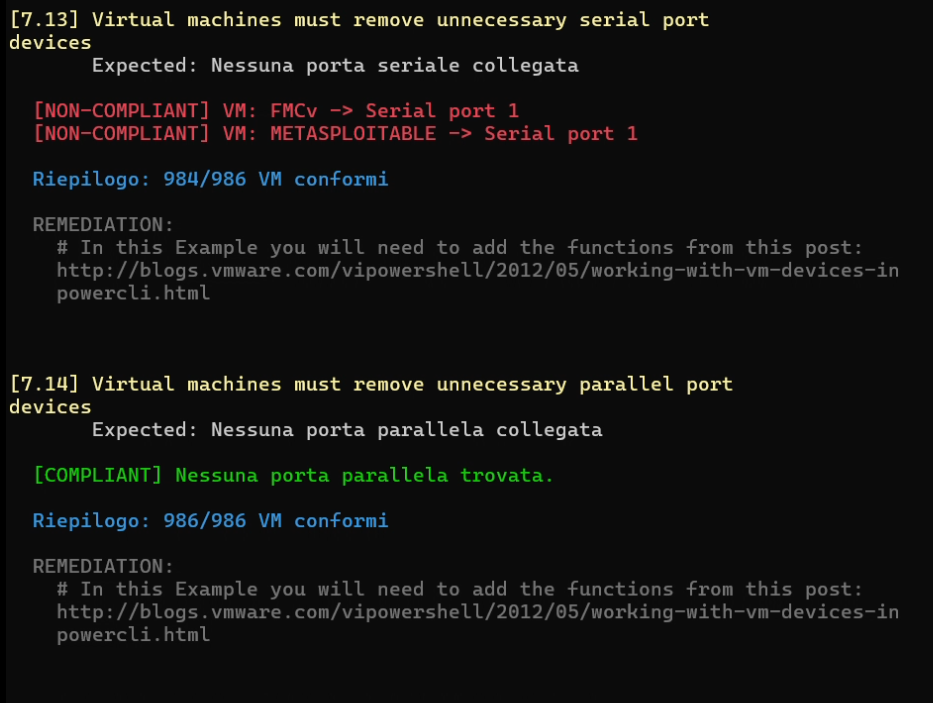
\includegraphics[width=0.9\textwidth]{esempio_comp}
    \caption{Esempio di output a console della valutazione dei controlli 7.13 e 7.14}
    \label{fig:screenshot-7-13-7-14}
\end{figure}




\section{Decisioni implementative rilevanti}

In questo paragrafo vengono evidenziate alcune scelte implementative rilevanti adottate durante lo sviluppo della soluzione. \\
Come citato alla fine del paragrafo precedente, è stato scelto di distinguere lo stato di non applicabilità del controllo rispetto alla conformità a prescindere. \\
Questa distinzione è resa esplicita nel report tramite un terzo stato dedicato, distinto da conforme e non conforme, ed escluso dal calcolo del tasso di conformità complessivo.\\
Questo perché essenzialmente il fatto di non avere nella propria infrastruttura oggetti valutabili per quello specifico controllo non implica la conformità o non conformità rispetto alla documentazione CIS. \\
Il risultato è che il tasso di conformità non venga ridotto artificialmente da controlli che non hanno prodotto una valutazione reale. \\

La gestione della sessione di autenticazione è stata gestita diversamente per i due ambienti.\\
Su Azure viene effettuata esternamente prima dell'esecuzione dello script principale, delegando l'autenticazione ai meccanismi nativi di Azure CLI, pensati per non richiedere che uno script terzo maneggi username e password. Il framework si limita a verificare che una sessione Azure sia già attiva, senza mai gestire credenziali direttamente. \\

Su VMware il discorso è diverso in quanto ci si collega durante l'esecuzione con un prompt interattivo. Questo perché è stato osservato durante lo sviluppo che la variabile globale \textit{\$global:DefaultVIServers}, utilizzata per verificare la presenza di una sessione attiva, non è risultata affidabile per lo scopo di questo progetto.


%			CAPITOLO 5: modello di scoring
\chapter{Il modello di scoring}

\section{Definizione delle dimensioni di effort: C, D, R}

Il modello di scoring utilizzato è stato definito durante la fase di progettazione e mira a valutare quantitativamente lo sforzo teorico necessario per risolvere la non conformità di un oggetto valutato dal tool. La valutazione si basa su tre valori che sono stati costruiti ad hoc e sono spiegati qui di seguito: C, D, R.\\

\begin{itemize}
\item C: complessità dell'intervento.\\
Questo parametro punta a quantificare quanto sia alto il costo in termini di procedure da svolgere per rendere l'oggetto conforme rispetto alla documentazione CIS. \\
L'intervallo dei valori ammissibili per C è \{1,2,3\}. La semantica dei valori è la seguente:
\begin{enumerate}
\item il tipo di operazioni coinvolte possono essere la semplice modifica di una proprietà di un oggetto che non alterano alcun componente dell'infrastruttura. Quindi una modifica parametrica locale.
\item l'intervento richiede di coordinare più componenti come ad esempio la creazione di una risorsa e il suo collegamento.
\item L'operazione qui è di tipo strutturale come ad esempio dover ricreare una virtual machine da zero per poter abilitare una certa funzionalità.
\end{enumerate}
\item D: indisponibilità. \\
Qui l'obiettivo è quantificare se l'intervento di remediation renda necessario o meno un fermo di qualche servizio.\\
L'intervallo dei valori ammissibili per D è \{0,1,2\}. La semantica dei valori è la seguente:
\begin{enumerate}[start=0]
\item Nessuna interruzione di servizio.
\item A seguito dell'intervento, è necessario un riavvio del servizio.
\item Per eseguire l'intervento è necessario un downtime di durata variabile, come ad esempio lo spegnimento di una virtual machine e il suo avvio da zero successivamente.
\end{enumerate}
\item R: reversibilità del rimedio. \\
Il terzo e ultimo parametro punta a quantificare la possibilità di fare rollback rispetto all'intervento di rimedio nel caso in cui si renda necessario per qualsiasi motivo(ad esempio un servizio che smette di funzionare). \\
L'intervallo dei valori ammissibili per R è \{1,2,3\}. La semantica dei valori è la seguente:
\begin{enumerate}
\item Reversibilità immediata. Ad esempio un singolo comando.
\item Reversibile con procedura strutturata. Può richiedere più passaggi e verifica di eventuali dipendenze.
\item Potenzialmente irreversibile. Può richiedere ricostruzione della risorsa da zero oppure il ripristino esatto non è garantito.
\end{enumerate}
\end{itemize}


L'assegnazione dei valori per ogni controllo CIS implementato è avvenuta mediante un'analisi qualitativa della documentazione. I parametri sono stati quindi inseriti, come già citato in precedenza, all'interno del dataset. In questo modo, al termine dell'esecuzione della valutazione, il software è in grado di attribuire lo sforzo per il rimedio a tutti gli oggetti non conformi leggendo i valori direttamente dal file csv di partenza. \\

\textit{A titolo dimostrativo, si mostrano tre esempi concreti tratti dal dataset Azure.} \\

\textbf{Controllo 2.3.6 -- Ensure 'HTTPS Only' is set to 'On' ($C=1$, $D=0$, $R=1$)}: in caso di non conformità l'intervento consiste nella modifica di una singola proprietà booleana (\texttt{httpsOnly}); non coinvolge quindi altre risorse, non richiede interruzione del servizio e può essere immediatamente invertito impostando nuovamente il valore precedente. \\

\textbf{Controllo 2.3.12 -- Ensure managed identities are configured ($C=1$, $D=0$, $R=2$)}: si tratta di un'operazione parametrica semplice ($C=1$), senza impatto sulla disponibilità del servizio ($D=0$). La reversibilità è tuttavia non banale. La rimozione dell'identità, se già utilizzata da altre risorse per l'accesso (ad esempio un Key Vault), può interrompere silenziosamente quelle integrazioni, rendendo necessaria una verifica delle dipendenze prima del rollback. \\

\textbf{Controllo 20.10 -- Ensure Trusted Launch is enabled on Virtual Machines ($C=3$, $D=2$, $R=3$)}: l'assegnazione qui dipende dalle assunzioni di partenza. Nel caso in cui la VM non fosse di gen 2, l'abilitazione di Trusted Launch su una macchina virtuale già esistente non è possibile, ma richiede la ricreazione della macchina con un nuovo profilo di sicurezza ($C=3$). Questo comporta chiaramente un'interruzione completa del servizio ($D=2$) e un eventuale rollback che equivale, a sua volta, a una nuova ricostruzione della macchina nello stato precedente ($R=3$).Tuttavia se invece la virtual machine fosse di gen 2 il valore di C scenderebbe a 2 poiché l'operazione richiederebbe la deallocazione della macchina e riconfigurazione, ma non la totale distruzione e ricreazione.\\

\textit{Analogamente, si riportano tre casi rappresentativi tratti dal dataset VMware.} \\


\textbf{Controllo 4.2 -- Host must transmit system logs to a remote log collector ($C=1$, $D=0$, $R=1$)}: la configurazione di un syslog remoto è un intervento che richiede tipicamente di configurare più impostazioni coordinate sull'host. L'operazione è priva di impatto sulla disponibilità delle macchine virtuali e immediatamente reversibile rimuovendo la configurazione impostata. \\

\textbf{Controllo 6.3.1 -- Host iSCSI client, if enabled, must employ bidirectional/mutual CHAP authentication ($C=2$, $D=1$, $R=2$)}: questo intervento richiede la configurazione coordinata delle credenziali sia sull'host ESXi sia sul target storage ($C=2$). La documentazione CIS segnala esplicitamente il rischio di interruzioni della comunicazione iSCSI qualora le credenziali configurate sui due lati non coincidano ($D=1$); il ripristino della configurazione precedente richiede una procedura strutturata di verifica su entrambi i lati della connessione ($R=2$). \\

\textbf{Controllo 3.21 -- Host should enable strict lockdown mode ($C=3$, $D=2$, $R=3$)}: questo esempio rappresenta il caso di effort massimo del dataset VMware. L'abilitazione di questa modalità può provocare l'impossibilità di accesso diretto all'host tramite Direct Console User Interface (DCUI), alterando la topologia di accesso amministrativo all'host ($C=3$) e potendo comportare un downtime critico ($D=2$) se non correttamente pianificata. Per quanto riguarda la reversibilità, la documentazione CIS segnala esplicitamente che il recupero da uno scenario simile può richiedere la reinstallazione dell'host ESXi. In determinati casi, il rollback può richiedere persino la presenza di un sistemista in datacenter per poter procedere alla reinstallazione dell'host ($R=3$).


\section{Definizione della metrica di effort E}


Le tre dimensioni definite nel paragrafo precedente sono state utilizzate per definire come segue una metrica di effort denominata $E$ per ogni controllo $i$ all'interno del dataset. \\


\begin{equation}
E_i = w_c \cdot C + w_d \cdot D + w_r \cdot R
\end{equation}


$w_c, w_d, w_r$ sono i valori dei pesi attribuiti ai tre valori C,D,R.\\
La somma di questi pesi deve essere tale che $w_c + w_d + w_r = 1$. \\

È quindi possibile modellare la metrica in funzione delle proprie necessità, come ad esempio pesare di più l'indisponibilità di servizio rispetto alla complessità procedurale dell'intervento. \\

La conseguenza di E definita in questo modo è che al variare dei pesi, le misurazioni non sono confrontabili tra loro. Di seguito viene mostrata una versione normalizzata della metrica, così che il suo valore sia sempre all'interno dell'intervallo [0,1] e confrontabile anche se vengono modificati i pesi. \\

\begin{equation}
E_{norm} = \frac{E_i - E_{min}}{E_{max} - E_{min}}
\end{equation}

$E_{min}$ ed $E_{max}$ sono i valori teorici minimi e massimi possibili.\\
$E_{min}$ rappresenta il caso più semplice possibile mentre $E_{max}$ rappresenta il caso più oneroso possibile. \\

\begin{equation}
E_{min} = w_c \cdot 1 + w_d \cdot 0 + w_r \cdot 1 
\end{equation}
\begin{equation}
E_{max} = w_c \cdot 3 + w_d \cdot 2 + w_r \cdot 3
\end{equation}


Si dimostra inoltre che il denominatore della normalizzazione è costante e pari a 2 indipendentemente dalla scelta dei pesi, essendo $w_c+w_d+w_r=1$ per costruzione.\\
\begin{align}
E_{max} - E_{min} &= w_c(3-1) + w_d(2-0) + w_r(3-1) \\
&= 2w_c + 2w_d + 2w_r = 2(w_c+w_d+w_r) = 2
\end{align}

La conseguenza di questa proprietà è che i controlli il cui profilo di effort soddisfa $(C-1)=D=(R-1)$ producono un valore di $E_{norm}$ costante, rispettivamente $0$, $0.5$ e $1$. Questo accade indipendentemente dalla scelta dei pesi sulle tre dimensioni C,D,R.\\

Possiamo quindi dire che per i profili simmetrici rispetto ai tre valori di effort, il modello di scoring si dimostra robusto rispetto ai pesi.

\subsection{Classificazione dell'effort in funzione di $E_{norm}$}

$E_{norm}$, una volta computato, viene tradotto in una classificazione a tre livelli tramite l'utilizzo di due soglie, $\alpha$ e $\beta$.\\


\begin{equation}
\text{Effort} =
\begin{cases}
\text{BASSO} & \text{se } E_{norm} < \alpha \\
\text{MEDIO} & \text{se } \alpha \leq E_{norm} < \beta \\
\text{ALTO}  & \text{se } E_{norm} \geq \beta
\end{cases}
\end{equation}

In questo caso di studio sono stati adottati i valori $\alpha = 0.35$ e $\beta = 0.7$. \\
Entrambe le soglie possono essere modificate in base alle proprie necessità, rendendo così più alto o più basso l'effort classificato dal framework. Questa classificazione a tre livelli è stata ideata per dare una lettura immediata sul costo del lavoro da svolgere, in combinazione al valore di $E_{norm}$. \\
Fondamentalmente BASSO indica un intervento di carattere contenuto e a basso impatto, MEDIO un intervento che richiede pianificazione e ALTO un intervento complesso con un impatto non indifferente.

%			CAPITOLO 6: esecuzione e analisi risultati
\chapter{Esecuzione framework e analisi risultati}

\section{Ambienti di test cloud e on-premise}

In questo paragrafo ci si soffermerà brevemente sugli ambienti di test utilizzati durante lo sviluppo.\\

Su \textbf{Microsoft Azure} è stata sfruttata la sottoscrizione Azure for Student grazie alle credenziali di ateneo. Una volta abilitato il profilo le operazioni eseguite sono state quelle di creare un numero limitato di risorse (Virtual Machines, Activity Log Alert, Web App, etc.etc.) con impostazioni minimali o di default ai soli fini di popolamento per poter essere poi sottoposte a valutazione dallo strumento sviluppato. \\

Su \textbf{VMware} invece come citato in un capitolo precedente è stato possibile utilizzare come ambiente di valutazione un'infrastruttura di laboratorio aziendale collocata presso Lutech S.p.A.\\
Si tratta di un ambiente non di produzione dedicato esclusivamente a sperimentazione di nuove soluzioni e/o per testare degli approcci prima dell'attività effettiva presso cliente. \\
Il sottoscritto stesso ha partecipato alla sua realizzazione sia nell'installazione fisica in datacenter che nella successiva configurazione degli host.\\
L'ambiente dispone di 14 host ESXi disposti su 4 cluster diversi su un vCenter, al momento con circa 1000 virtual machines.\\
Considerata l'ampiezza dell'infrastruttura, l'esito della reportistica per VMware ha coinvolto un numero di oggetti significativamente maggiore rispetto ad Azure, rendendo l'analisi statistica sulla distribuzione dell'effort più solida su questa piattaforma.


\section{Analisi dei risultati}

L'esecuzione del framework su Azure ha valutato una totalità di 60 controlli previsti dal dataset popolato. È stato riscontrato un tasso di conformità del 28.3\%, con 17 controlli conformi su 60. \\
La distribuzione dei controlli non conformi è concentrata nella fascia di effort BASSO con 29 controlli, seguita dalla fascia MEDIO con 11 occorrenze e infine ALTO con sole tre verifiche non conformi. \\
In questa casistica specifica possiamo evincere che la maggioranza degli interventi di remediation che si rendono necessari per risultare conformi richieda un costo basso e ragionevole.\\ 

\begin{figure}[H]
	\centering
	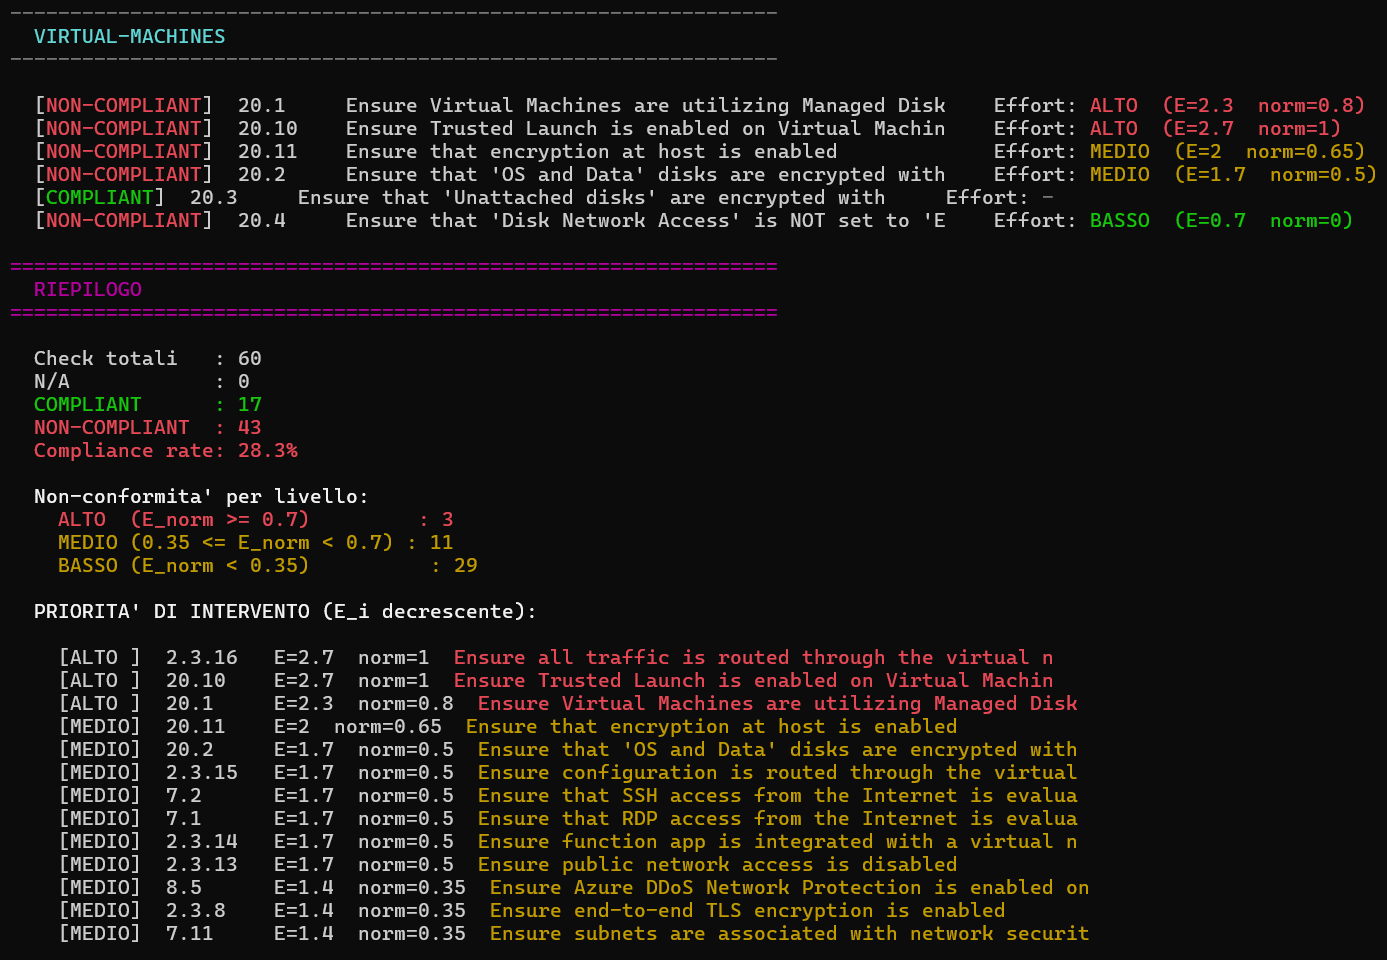
\includegraphics[width=1.0\textwidth]{report_azure}
    \caption{Estratto del riepilogo finale di esecuzione su Azure}
    \label{fig:report_azure}
\end{figure}


Per quanto riguarda invece l'esecuzione su VMware, sono stati valutati una totalità di 39 controlli sempre previsti dal dataset costruito inizialmente. Qui è stato registrato un tasso di conformità del 41\%, con 16 controlli conformi su 39.\\
Anche in questo la maggior parte degli interventi necessari sono rientrati nella fascia BASSO, con solo due non conformità nella fascia MEDIO e uno su ALTO.\\ 

\begin{figure}[H]
	\centering
	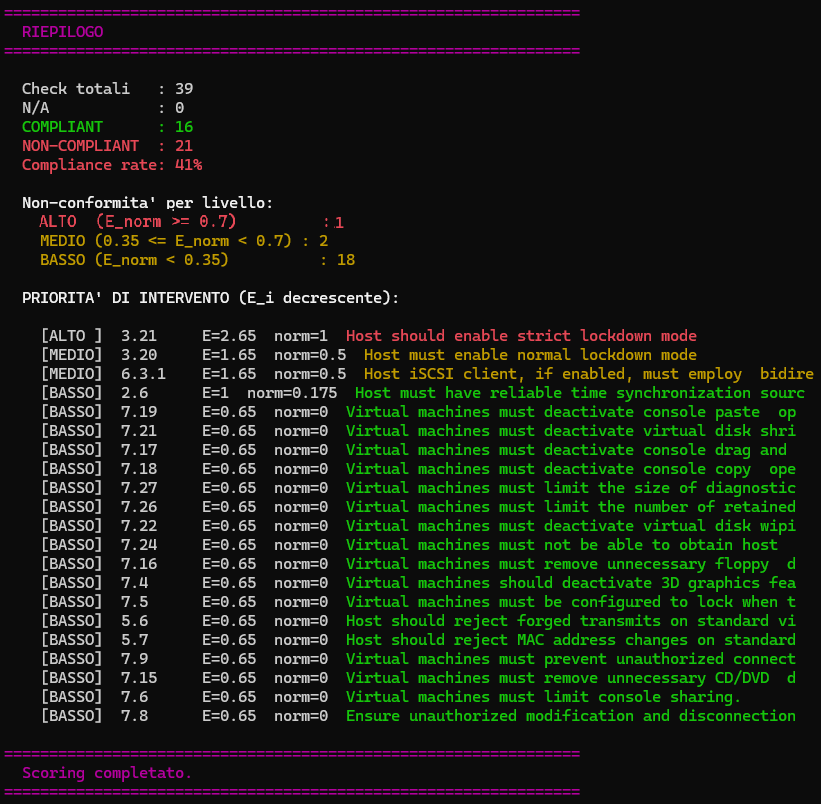
\includegraphics[width=1.0\textwidth]{report_vmware}
    \caption{Estratto del riepilogo finale di esecuzione su VMware}
    \label{fig:report_vmware}
\end{figure}

Per approfondire la lettura dei risultati finora presentati, è stato costruito un diagramma che incrocia l'effort di remediation calcolato con $E_{norm}$ con l'impatto reale di ciascun controllo, inteso come il numero di oggetti coinvolti dalla non conformità sull'infrastruttura.\\
Grazie a questa rappresentazione è possibile distinguere dei controlli che a parità di effort coinvolgono un numero diverso di risorse.\\
Ad esempio un controllo che richiede interventi a basso costo che però vede coinvolte molte risorse rappresenta in questo grafico un intervento di priorità più alta, poiché facilmente risolvibile per molti oggetti. Viceversa un controllo che richiede interventi complessi ma con poche risorse coinvolte, in questo grafico ha minore priorità in quanto andrebbe pianificato con più cura.\\

Il grafico è suddiviso in quattro quadranti da  due soglie. La linea tratteggiata verticale rappresenta la soglia $\beta$ introdotta nel corso del capitolo 5, mentre la linea tratteggiata orizzontale rappresenta la mediana del numero di oggetti non conformi riscontrati. \\

Incrociando le due linee, i quadranti sono divisi come segue:
\begin{itemize}
\item Primo quadrante. \\
In alto a destra vi sono i punti con effort alto e impatto alto. Qui vi cadono quei controlli non conformi che richiedono interventi complessi, ma che allo stesso tempo hanno rilevato molte risorse non in linea con i benchmark. In questo caso il team operativo dovrebbe pianificare con cura la risoluzione programmando una finestra di manutenzione.
\item Secondo quadrante. \\
In alto a sinistra troviamo molti controlli non conformi con costo basso di remediation.
\item Terzo quadrante. \\
Qui troviamo controlli non conformi il cui effort di risoluzione è basso, ma anche il numero di oggetti coinvolti è basso.
\item Quarto quadrante. \\
In questa area del grafico troviamo le valutazioni non conformi meno convenienti da risolvere nell'immediato. Questo poichè abbiamo pochi oggetti con costo di intervento alto.
\end{itemize}


La Figura \ref{fig:diagramma-azure} riporta il diagramma prodotto per l'ambiente Azure. Dato il numero esiguo di risorse create sull'infrastruttura di test con la sottoscrizione da studente, l'asse delle y rappresentativo dell'impatto risulta chiaramente contenuto(compreso tra 1 e 3 oggetti). \\


\begin{figure}[H]
	\centering
	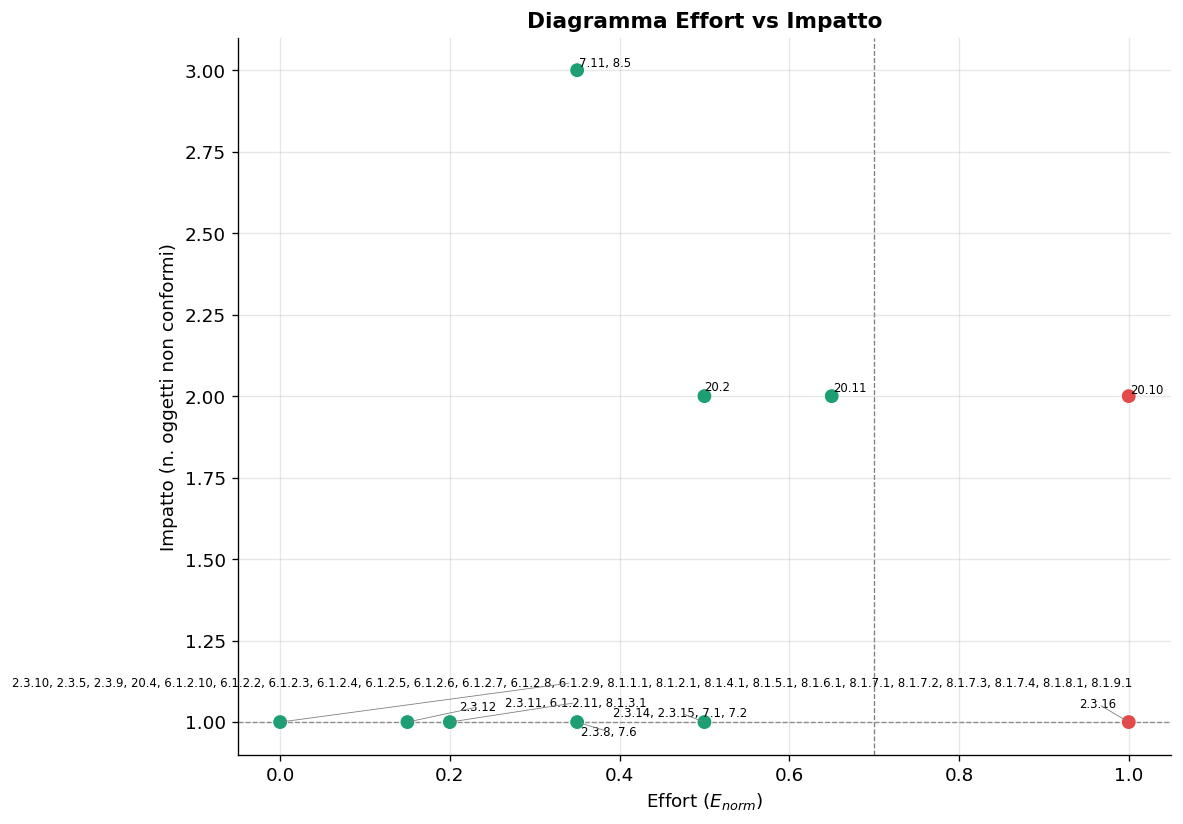
\includegraphics[width=1\textwidth]{Effort_Impact_Matrix_azure}
    \caption{Diagramma di confronto tra effort e impatto -- ambiente Azure}
    \label{fig:diagramma-azure}
\end{figure}


La Figura \ref{fig:diagramma-vmware} riporta il diagramma prodotto per l'ambiente VMware. A differenza di Azure, avendo avuto qui un'infrastruttura molto più grande, l'impatto della non conformità raggiunge di conseguenza valori significativamente più elevati. Questo fa si che la dimensione dell'impatto sia più rilevante rispetto al grafico precedente per quanto riguarda l'identificazione delle priorità di intervento. \\


\begin{figure}[H]
	\centering
	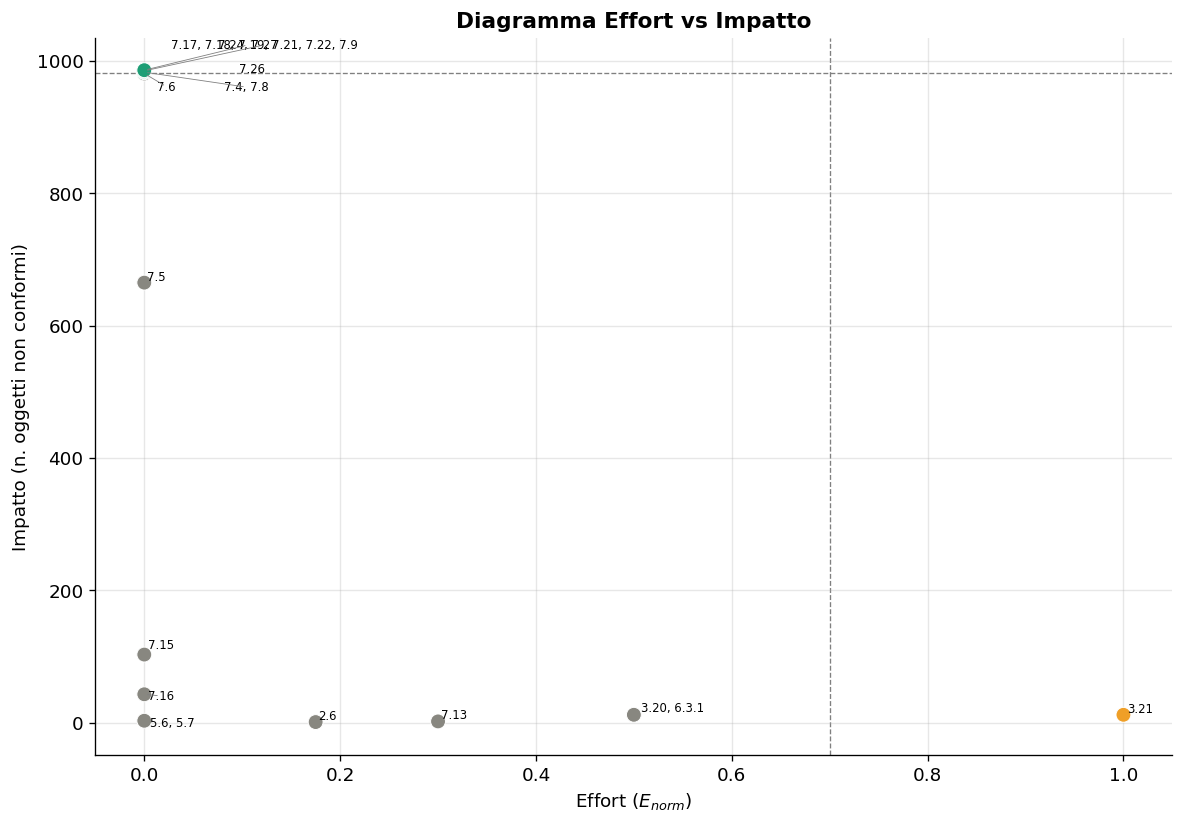
\includegraphics[width=1\textwidth]{Effort_Impact_Matrix_vmware}
    \caption{Diagramma di confronto tra effort e impatto -- ambiente VMware}
    \label{fig:diagramma-vmware}
\end{figure}


\section{Differenze strutturali nei benchmark Azure e VMware}

In questo paragrafo viene confrontata la struttura dei due benchmark utilizzati a livello di definizione dei controlli, escludendo i risultati osservati sulle rispettive infrastrutture di test. Il confronto opera sui valori $E_{norm}$ derivati dai parametri C, D, R assegnati a ciascun controllo sui dataset iniziali.\\
La distribuzione di $E_{norm}$ sui 60 controlli del dataset Azure e sui 39 controlli del dataset VMware è riportata in Figura~\ref{fig:confronto_benchmark}, tramite boxplot e conteggio dei controlli per valore di $E_{norm}$ su grafico a barre.


\begin{figure}[H]
	\centering
	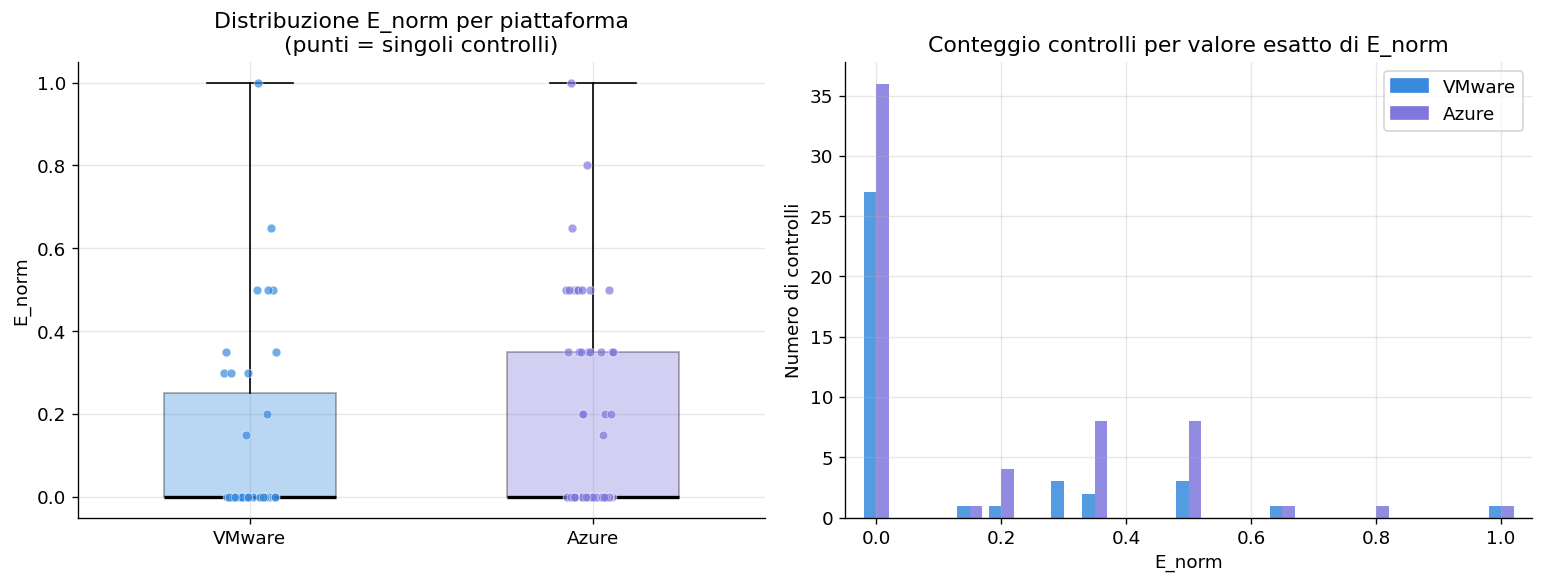
\includegraphics[width=1.0\textwidth]{confronto_benchmark.png}
    \caption{Distribuzione di $E_{norm}$ a confronto tra i dataset Azure e VMware}
    \label{fig:confronto_benchmark}
\end{figure}

In entrambi i casi la mediana di $E_{norm}$ coincide con il valore minimo possibile, pari a zero, indicando che almeno la metà dei controlli selezionati di ciascun ambiente presenta il livello di effort più basso possibile.\\
Sul boxplot è possibile osservare che i pochi controlli con effort elevato compaiono come punti isolati nella parte superiore del grafico.\\
Si osserva inoltre che la sovrapposizione della mediana con il bordo inferiore della scatola del boxplot è conseguenza diretta della forte concentrazione di controlli a $E_{norm}=0$, che supera il 25\% della distribuzione in entrambi i casi.\\

Nel grafico a barre sulla destra è riportato il numero di controlli per ciascun valore di $E_{norm}$. \\
In generale, la rappresentazione evidenzia una forte concentrazione di controlli a $E_{norm}=0$ per entrambe le piattaforme (36 su 60 per Azure, 27 su 39 per VMware), seguita da un numero contenuto di controlli distribuito sui restanti valori discreti ammissibili. Il valore massimo $E_{norm}=1$ risulta raggiunto da un solo controllo per piattaforma.\\

Considerando la natura della popolazione di controlli utilizzata, non è stato applicato un test di verifica di ipotesi.\\
I controlli VMware e Azure all'interno dei due dataset in questione non rappresentano un campione estratto in modo totalmente casuale dalla popolazione iniziale, bensì l'insieme delle verifiche di conformità selezionate e implementate durante questo lavoro secondo criteri di copertura pratica. \\
Un eventuale risultato del test non potrebbe essere generalizzato all'intero standard CIS di ciascuna piattaforma. Tale confronto è quindi limitato al piano descrittivo, come mostrato in Figura~\ref{fig:confronto_benchmark}.

%			CAPITOLO 7: Guida operativa passo passo
\chapter{Guida operativa all'utilizzo}

Questo capitolo mira a fornire una guida per l'utilizzo del framework su un proprio ambiente e all'interpretazione dei file di output prodotti.
Ci si focalizzerà quindi sugli aspetti operativi, quali la preparazione dell'ambiente, i parametri di lancio del software, i file prodotti e le situazioni di errore più comuni.

\section{Preparazione dell'ambiente di esecuzione}

Per poter eseguire il framework è sufficiente avere a disposizione un terminale con PowerShell installato.
Il software non richiede alcun tipo di installazione, bisogna solo disporre della cartella di progetto con all'interno il sorgente. Le uniche dipendenze da dover installare se assenti sono Azure CLI e il modulo VMware PowerCLI.\\
I requisiti di autenticazione sono già stati descritti nel paragrafo 3.3.

I percorsi vengono risolti partendo dalla posizione degli script PowerShell. Data questa premessa, la struttura del progetto va mantenuta come segue:


\begin{table}[H]
\centering
\small
\begin{tabular}{p{4.6cm}p{7cm}}
\hline
\textbf{Elemento} & \textbf{Contenuto} \\
\hline
\texttt{Analisi\_Report/} & \texttt{main\_azure.ps1}, \texttt{main\_vmware.ps1}, \texttt{module\_scoring.ps1} \\ \hline
\texttt{Azure/} & un modulo per ciascuna sezione del benchmark Azure implementata \\ \hline
\texttt{VMware/} & un modulo per ciascuna sezione del benchmark VMware implementata \\ \hline
\texttt{module\_utils.ps1} & funzioni condivise (inizializzazione, registrazione dei risultati) \\ \hline
\texttt{cis\_azure.csv}, \texttt{cis\_vmware.csv} & dataset dei controlli \\ 
\hline
\end{tabular}
\caption{Struttura della cartella del progetto}
\label{tab:struttura}
\end{table}

Nel caso in cui le impostazioni del sistema dovessero impedire l'esecuzione di script non firmati, è possibile aggirare la policy per il singolo processo mediante il seguente comando.

\begin{lstlisting}[style=azcli]
powershell -ExecutionPolicy Bypass -File ".\main_azure.ps1"
Oppure
powershell -ExecutionPolicy Bypass -File ".\main_vmware.ps1"
\end{lstlisting}

Dal momento che il software si limita solo a leggere la configurazione dell'ambiente, l'account utilizzato non necessita di permessi di scrittura sulle risorse di cui va a valutare la conformità rispetto al benchmark.\\
I comandi mostrati in output relativi alle remediation provengono dal dataset e sono riportati solo come suggerimento, non vengono mai eseguiti.

\section{Avvio esecuzione}

È necessaria una sessione attiva sulla piattaforma di cui si intende lanciare la valutazione di conformità. Il framework non ha una gestione delle credenziali(paragrafo 4.3).

Per Azure è sufficiente quanto segue:

\begin{lstlisting}[style=azcli]
az login
az account set --subscription "<nome o id>"
.\main_azure.ps1
\end{lstlisting}

Il secondo comando riportato si rende necessario nella casistica in cui l'account abbia accesso a molteplici sottoscrizioni e quella predefinita non sia quella che si vuole utilizzare.

Su VMware invece il comando è il seguente:

\begin{lstlisting}[style=azcli]
Connect-VIServer -Server <fqdn-vCenter> _User <username> -Password <password>
.\main_vmware.ps1
\end{lstlisting}

Il tool, tra le prime azioni che compie, procede a verificare subito la presenza di una sessione attiva sulla piattaforma che sta per valutare.\\
Su Azure, se avviene con successo la verifica, viene stampato a schermo il nome dell'account e la sottoscrizione che verrà utilizzata dal software per l'analisi dell'infrastruttura. Oltre a ciò viene anche mostrato il numero di controlli caricati dal dataset utilizzato.\\
Su VMware l'output a schermo è similare e viene mostrato il vCenter al quale si è connessi.

In questo modo è possibile accorgersi fin da subito se si è collegati all'ambiente errato prima ancora dell'esecuzione dei controlli.

La console, durante l'esecuzione, mostra a schermo diverse informazioni nel seguente ordine:

\begin{enumerate}
\item l'esito della valutazione di ciascun controllo, raggruppato per modulo (si veda la Figura 4 nel capitolo 4 per un esempio).
\item Un riepilogo complessivo sullo stato della situazione a controlli eseguiti, nel formato \texttt{RIEPILOGO: x/y COMPLIANT}.
\item l'output a seguito della computazione dello scoring. Viene mostrato l'elenco dei controlli per categoria con stato di conformità ed effort (Per un esempio rivedere le Figure 5 e 6 nel capitolo 6). In coda, vi è anche l'elenco delle non conformità ordinato per valore decrescente di $E_i$.
\end{enumerate}


\section{Parametri esistenti}

Gli script di entrambi gli ambienti accettano gli stessi parametri, i quali vengono riassunti nella tabella~\ref{tab:parametri}

\begin{table}[H]
\centering
\small
\begin{tabular}{p{2.3cm}p{3.1cm}p{6.2cm}}
\hline
\textbf{Parametro} & \textbf{Predefinito} & \textbf{Effetto} \\
\hline
\texttt{-AuditOnly} & disattivato & Esegue solo i controlli, senza calcolo dello scoring né esportazione del report. \\ \hline
\texttt{-ExportLog} & disattivato & Salva in un file di testo l'intero output della console. \\ \hline
\texttt{-Wc -Wd -Wr} & 0.30, 0.40, 0.30 & Pesi di C, D, R nella metrica $E_i$. Devono sommare a 1. \\ \hline
\texttt{-Alpha -Beta} & 0.35, 0.70 & Soglie di classificazione dell'effort. Alpha deve essere minore di Beta. \\ \hline
\texttt{-CsvPath} & dataset nella cartella radice & Percorso alternativo del dataset. \\ \hline
\texttt{-OutputDir} & cartella \texttt{Analisi\_Report} & Cartella in cui viene scritto il file di log. \\
\hline
\end{tabular}
\caption{Tabella riassuntiva sui parametri utilizzabili da linea di comando.}
\label{tab:parametri}
\end{table}

Di seguito vengono mostrati quindi alcuni esempi di invocazione:

\begin{lstlisting}[style=azcli]
.\main_azure.ps1 -AuditOnly
.\main_azure.ps1 -ExportLog
.\main_vmware.ps1 -Wc 0.5 -Wd 0.3 -Wr 0.2
.\main_vmware.ps1 -Wc 0.5 -Wd 0.3 -Wr 0.2 -Alpha 0.3 -Beta 0.65
.\main_vmware.ps1 -ExportLog -OutputDir "C:\reports"
\end{lstlisting}

\section{Output riportato e struttura del report}
\label{sec:file}

Alla conclusione dell'esecuzione vengono prodotti fino a tre file, descritti di seguito.

\begin{itemize}
\item il \textbf{log di sessione}, con nome \texttt{cis\_azure\_log\_<data\_ora>.txt} oppure \texttt{cis\_vmware\_log\_<data\_ora>.txt}, solo se è stata usata l'opzione \texttt{-ExportLog}.
\item il \textbf{report dei controlli}, \texttt{cis\_scoring\_report\_<data\_ora>.csv}, con una riga per ciascun controllo del dataset.
\item il \textbf{riepilogo}, con lo stesso nome del report seguito da \texttt{\_summary}, composto da una sola riga.
\end{itemize}

I file relativi al report e riepilogo vengono salvati nella directory in cui è posizionato il terminale, mentre \texttt{-OutputDir} riguarda solo il file di log. Utilizzando l'opzione \texttt{-AuditOnly} nessuno dei due file (report/riepilogo) viene prodotto.

La seguente tabella riporta e descrive le colonne presenti all'interno del report.

\begin{table}[H]
\centering
\small
\begin{tabular}{p{2.7cm}p{8.9cm}}
\hline
\textbf{Colonna} & \textbf{Contenuto} \\
\hline
\texttt{ID}, \texttt{Category}, \texttt{Name} & Identificativo CIS, categoria e titolo del controllo, esattamente come all'interno del dataset. \\ \hline
\texttt{Status} & \texttt{COMPLIANT}, \texttt{NON-COMPLIANT}, \texttt{N/A} oppure \texttt{UNKNOWN}. \\ \hline
\texttt{Total} & Numero di oggetti valutati dal controllo. \\ \hline
\texttt{NonCompliant} & Numero di oggetti non conformi tra quelli valutati. \\ \hline
\texttt{C}, \texttt{D}, \texttt{R} & Valori di complessità, indisponibilità e reversibilità dell'intervento di remediation letti dal dataset. \\ \hline
\texttt{E\_i}, \texttt{E\_norm} & Effort calcolato con i pesi in uso e versione normalizzata. \\ \hline
\texttt{Effort} & Fascia assegnata: \texttt{BASSO}, \texttt{MEDIO} o \texttt{ALTO}. \\ \hline
\texttt{Objects} & Identificativi degli oggetti non conformi, separati dal carattere \texttt{|}. \\ \hline
\texttt{Remediation} & Procedura di rimedio indicata dal benchmark per quel controllo. \\ 
\hline
\end{tabular}
\caption{Descrizione del contenuto all'interno del report prodotto in output.}
\label{tab:colonne}
\end{table}

Un dettaglio rilevante rigurda il valore di stato \texttt{UNKNOWN}. Tale statement viene assegnato nel caso in cui la valutazione di un controllo di conformità non ha registrato alcun risultato. Questo può succedere quando il modulo in questione è stato saltato e non eseguito(ad esempio se la logica di audit di un controllo richiedesse una verifica manuale).\\
Diversa è la semantica rispetto a \texttt{N/A}, il quale ci indica che il controllo è stato eseguito ma all'interno dell'infrastruttura non vi era alcun oggetto da valutare.

Le colonne relative alla metrica di Effort vengono valorizzate in modo significativo solo per i controlli che sono risultati non conformi. 

Il file di riepilogo contiene solamente i totali dell'esecuzione. Quindi il nome della piattaforma valutata, il numero di controlli coinvolti, conformi e non conformi. Oltre a ciò viene indicata una percentuale di conformità e il totale di componenti non conformi per ogni fascia di effort.
Entrambi i file di report/riepilogo sono in formato CSV, consultabili mediante foglio di calcolo con cui è possibile eseguire filtri e analizzare i risultati.

\section{Situazioni di errore comuni}

Nella tabella ~\ref{tab:errori} si procede ad elencare in sintesi le situazioni di errore più comuni che si possono incontrare e il comportamento che ha il framework.

\begin{table}[H]
\centering
\small
\renewcommand{\arraystretch}{1.35}
\begin{tabularx}{\textwidth}{
  >{\raggedright\arraybackslash}p{0.24\textwidth}
  >{\raggedright\arraybackslash}X
  >{\raggedright\arraybackslash}p{0.27\textwidth}}
\hline
\textbf{Situazione} & \textbf{Comportamento} & \textbf{Azione} \\
\hline
Sessione Azure o vCenter assente & L'esecuzione termina con un messaggio prima di avviare qualsiasi controllo. & Eseguire \texttt{az login} o \texttt{Connect-VIServer}. \\ \hline
Dataset non trovato & L'esecuzione termina con un avviso di errore. & Verificare la struttura delle cartelle o indicare \texttt{-CsvPath}. \\ \hline
Pesi con somma diversa da 1, oppure Alpha non minore di Beta & I controlli vengono eseguiti e mostrati a console, ma la fase di scoring termina con un errore e il report non viene prodotto. & Correggere i parametri e rilanciare. \\ \hline
File di un modulo mancante & Il modulo viene saltato con un avviso e l'esecuzione prosegue. I suoi controlli risulteranno \texttt{UNKNOWN}. & Ripristinare il file. \\ \hline
Esecuzione script bloccata & Il sistema rifiuta l'esecuzione dello script. & Utilizzare l'opzione \texttt{-ExecutionPolicy Bypass}. \\
\hline
\end{tabularx}
\caption{Errori comuni e comportamento del framework}
\label{tab:errori}
\end{table}


Siccome la validazione dei pesi e delle soglie avviene solamente in fase di scoring, è consigliabile verificare con attenzione quando vengono modificati rispetto ai valori predefiniti.
Questo problema non si pone nell'ambito dell'integrazione del framework sulla piattaforma Moon Cloud, descritta nel capitolo successivo.

% 			CAPITOLO 8: integrazione sonda Moon Cloud
\chapter{Integrazione nell'ambiente Moon Cloud}


\section{Contesto e obiettivo}

Una volta che è stato ultimato il framework finora presentato, è stato possibile effettuare la sua integrazione con l'ambiente Moon Cloud.\\
Moon cloud~\cite{Anisetti2018} è una piattaforma dedicata per la verifica della conformità di applicazioni e infrastrutture in grado di eseguire una valutazione continua durante il loro intero ciclo di vita.

Questa piattaforma esegue periodicamente delle \textit{sonde} (\textit{probe}), quindi componenti software indipendenti, ciascuna incaricata di verificare la conformità di uno specifico aspetto di sicurezza su un componente target(applicazione o infrastruttura), restituendo al termine un esito strutturato dei controlli eseguiti.

In questo modo il framework per la valutazione di conformità agli standard CIS, oltre ad essere eseguibile localmente, può anche fare parte di un processo di monitoraggio continuo dell'infrastruttura.
Chiaramente l'obiettivo qui non è stato la riscrittura dell'intero strumento in funzione di Moon Cloud, bensì la costruzione di un adattatore che ne rispetti i requisiti di funzionalità, andando a riutilizzare la stessa logica di audit e di scoring già sviluppata.

Un ulteriore precisazione è che l'integrazione del framework verso questo ambiente è stata realizzata solamente per quanto riguarda le funzionalità sviluppate per Microsoft Azure. 

\section{Le specifiche di Moon Cloud: la sonda come macchina a stati}

Ogni sonda che viene sviluppata è eseguita dal driver di Moon Cloud, trattasi di una libreria Python installata nell'immagine Docker della sonda. Il driver riceve in ingresso i parametri dell'esecuzione e li valida rispetto a uno schema. Successivamente esegue in ordine i passi strutturati nella sonda, gestisce le eccezioni che questi potrebbero sollevare e infine restituisce alla piattaforma il risultato ottenuto.\\
Per sviluppare una sonda ci si occupa solamente di implementare i passi che il driver richiama.

Il requisito principale richiesto dal driver Moon Cloud consiste nel fatto che ogni sonda sia implementata come una classe Python che eredita da \texttt{AbstractProbe}, strutturata come una macchina a stati finiti.\\
Vi è una sequenza di \textit{atomi} (\textit{atoms}), ognuno dei quali costituito da una coppia di funzioni:
\begin{itemize}
\item \textit{forward}.
Viene eseguita nel normale flusso di esecuzione.
\item \textit{rollback}.
Viene invocata solo in caso di errore per disfare eventuali effetti collaterali.
\end{itemize}

L'esecuzione quindi inizia nel flusso \textit{forward}, un atomo dopo l'altro. Nel caso in cui si dovesse verificare un errore, in funzione di come è stato definito all'interno dello specifico atomo, l'esecuzione può arrestarsi oppure passare al flusso di \textit{rollback}.

Per ogni atomo vengono definite le eccezioni da intercettare, l'azione da intraprendere se una di esse viene sollevata e la funzione che ha il compito di costruire il messaggio da restituire.\\
Ad esempio l'azione da intraprendere può essere \texttt{STOP}, dunque l'interruzione dell'esecuzione con restituzione immediata del risultato costruito per quell'errore. In un altro caso può essere \texttt{ROLLBACK} che consiste nell'avviare il flusso di rollback prima di restituire il risultato.

Di seguito è riportata la definizione completa del metodo \texttt{atoms()}. Tale definizione è comune a tutte le sonde sviluppate.

\begin{lstlisting}[style=azcli, caption={Definizione di atoms per ogni sonda sviluppata.}, label={lst:atoms}]
def atoms(self) -> typing.Sequence[atom.AtomPairWithException]:
    return [
        atom.AtomPairWithException(
            forward=self.init,
            forward_captured_exceptions=[
                atom.PunctualExceptionInformationForward(
                    exception_class=AssertionError,
                    action=atom.OnExceptionActionForward.STOP,
                    result_producer=self._input_error,
                ),
                atom.PunctualExceptionInformationForward(
                    exception_class=ValueError,
                    action=atom.OnExceptionActionForward.STOP,
                    result_producer=self._input_error,
                ),
            ],
        ),
        atom.AtomPairWithException(
            forward=self.azure_login,
            forward_captured_exceptions=[
                atom.PunctualExceptionInformationForward(
                    exception_class=Exception,
                    action=atom.OnExceptionActionForward.ROLLBACK,
                    result_producer=self._connection_error,
                ),
            ],
            rollback=self.rollback_azure_login,
        ),
        atom.AtomPairWithException(
            forward=self.run_audit,
            forward_captured_exceptions=[
                atom.PunctualExceptionInformationForward(
                    exception_class=ConnectionError,
                    action=atom.OnExceptionActionForward.ROLLBACK,
                    result_producer=self._connection_error,
                ),
                atom.PunctualExceptionInformationForward(
                    exception_class=Exception,
                    action=atom.OnExceptionActionForward.ROLLBACK,
                    result_producer=self._execution_error,
                ),
            ],
            rollback=self.rollback_azure_login,
        ),
        atom.AtomPairWithException(
            forward=self.make_result,
            forward_captured_exceptions=[
                atom.PunctualExceptionInformationForward(
                    exception_class=Exception,
                    action=atom.OnExceptionActionForward.STOP,
                    result_producer=self._execution_error,
                ),
            ],
        ),
    ]
\end{lstlisting}

La struttura della funzione atoms è quindi composta da quattro atomi, ognuno dei quali verrà descritto nei successivi paragrafi.
\begin{itemize}
\item \texttt{init}
\item \texttt{azure\_login}
\item \texttt{run\_audit}
\item \texttt{make\_result}
\end{itemize}

Nel caso d'uso di questo progetto, solo l'atomo \texttt{azure\_login} dispone di un rollback, poichè è l'unico passaggio che produce uno stato persistente al di fuori del ciclo di vita della singola esecuzione. Trattasi della sessione Azure CLI autenticata.


\section{Riutilizzo del framework via processo esterno}

Un primo approccio per la realizzazione delle sonde sarebbe potuto essere la riscrittura della logica in Python, in modo tale da evitare dipendenze esterne.
Questa opzione è stata fin da subito scartata per due motivazioni.
\begin{enumerate}
\item Il framework PowerShell descritto nei capitoli precedenti era già stato validato e testato su un paio di infrastrutture.
Tradurre l'intero strumento in un altro linguaggio sarebbe risultato oneroso e avrebbe potuto introdurre altresì rischi di errori su funzionalità già corrette e testate.
\item La documentazione del driver Moon Cloud prevede in modo esplicito la possibilità di invocare uno strumento esterno all'interno di una sonda Python. Data questa possibilità, l'architettura scelta si inserisce in una modalità di integrazione già prevista. PowerShell viene quindi installato all'interno del container come dipendenza esterna.
\end{enumerate}

Il costo di questa scelta architetturale ricade sulla dimensione dell'immagine Docker, chiaramente più pesante rispetto a una sonda nativa Python a causa delle dipendenze esterne da dover installare. Trattasi di un compromesso ritenuto accettabile a fronte del riutilizzo di uno strumento già ultimato.

\section{Architettura della sonda}

Di seguito in Figura~\ref{fig:architettura-sonda} viene illustrato il flusso complessivo di esecuzione di una singola sonda. 

La piattaforma Moon Cloud, esterna al container, invia l'input al driver, il quale procede a validarlo e avvia la sonda.\\
Vengono quindi eseguiti in sequenza i quattro atomi. Il framework PowerShell interroga Azure e restituisce l'esito alla sonda, che a sua volta consegna il risultato al driver e da li alla piattaforma.

La sonda Python (\texttt{probe.py}) autentica la sessione Azure CLI e successivamente invoca come sottoprocesso uno script PowerShell (\texttt{probe\_runner.ps1}) che ha il compito di orchestrare l'esecuzione del framework esistente.
Al termine, viene prodotto un file JSON con l'esito della valutazione.


\begin{figure}[H]
	\centering
	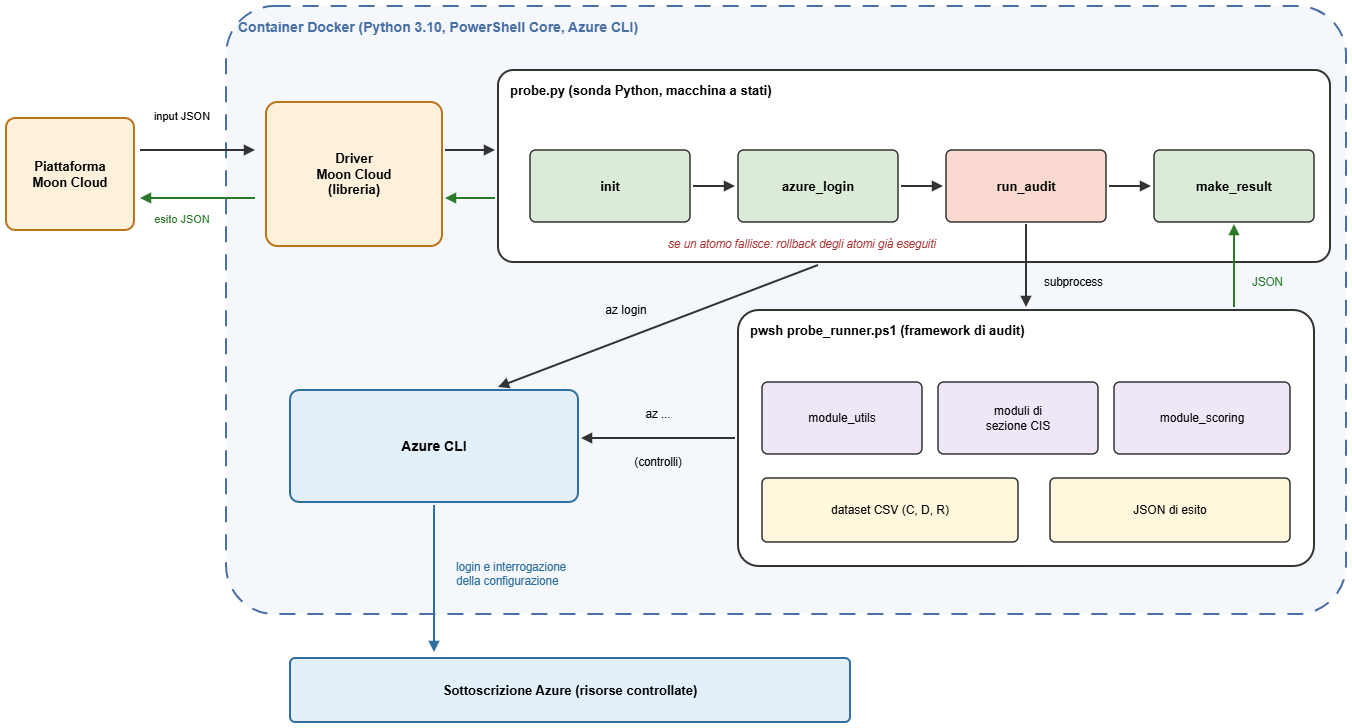
\includegraphics[width=1.0\textwidth]{architettura_sonda_moon_cloud}
    \caption{Flusso di esecuzione di una sonda Moon Cloud integrata con il framework PowerShell.}
    \label{fig:architettura-sonda}
\end{figure}



I successivi quattro paragrafi vanno a decrivere ciascun atomo che compone la sonda.

\subsection{init: validazione dell'input}

L'atomo init ha la funzione di leggere e validare i dati necessari all'esecuzione del framework, quindi l'input e le credenziali Azure. Vengono letti tre gruppi di parametri dall'input fornito. Il gruppo \texttt{config} contiene l'identificativo della sottoscrizione Azure.
il gruppo \texttt{audit} contiene il tempo massimo concesso per l'esecuzione( di default 1800 secondi).
Il gruppo \texttt{scoring} contiene i pesi $w_c$, $w_d$, $w_r$ e le soglie $\alpha$ e $\beta$, con i valori di default utilizzati dalla sonda.
Le credenziali del service principal (\texttt{tenant\_id}, \texttt{client\_id}, \texttt{client\_secret}) sono lette dal file dedicato.

La seguente porzione di codice ne riporta l'implementazione.


\begin{lstlisting}[style=azcli, caption={Atomo \texttt{init}: validazione dell'input e delle credenziali}, label={lst:init}]
def init(self, inputs: typing.Any = None) -> bool:
    config = self.config.input.get("config") or {}

    # validazione sottoscrizione azure
    self.subscription_id = config.get("subscription_id", "")
    assert self.subscription_id, "Il campo 'config.subscription_id' e' obbligatorio"

    audit = self.config.input.get("audit") or {}
    self.timeout = int(audit.get("timeout_seconds", self.DEFAULT_TIMEOUT))

    # validazione pesi per lo scoring finale
    scoring = self.config.input.get("scoring") or {}
    wc = float(scoring.get("wc", 0.40))
    wd = float(scoring.get("wd", 0.30))
    wr = float(scoring.get("wr", 0.30))
    assert abs(wc + wd + wr - 1.0) < 0.001, (
        f"I pesi devono sommare a 1.0 (attuale: {round(wc + wd + wr, 4)})"
    )
    self.weights = {"wc": wc, "wd": wd, "wr": wr}

    alfa = float(scoring.get("alfa", 0.35))
    beta = float(scoring.get("beta", 0.70))
    assert 0.0 <= alfa < beta <= 1.0, (
        f"Soglie non valide: richiesto 0 <= alfa < beta <= 1 (alfa={alfa}, beta={beta})"
    )
    self.thresholds = {"alfa": alfa, "beta": beta}

    # verifica credenziali in credential.json
    credential = self.config.credential or {}
    self.tenant_id = credential.get("tenant_id", "")
    self.client_id = credential.get("client_id", "")
    self.client_secret = credential.get("client_secret", "")
    assert self.tenant_id and self.client_id and self.client_secret, (
        "Credenziali incomplete: servono 'tenant_id', 'client_id' e 'client_secret' "
        "di un service principal Azure con ruolo Reader sulla subscription"
    )

    self.json_path = os.path.join(tempfile.gettempdir(), "cis_azure_result.json")
    return True
\end{lstlisting}


È da notare come i vincoli del modello di scoring illustrati e discussi nel capitolo 5, quindi la somma dei pesi a 1 e le soglie    $\alpha < \beta$, vengono verificati fin da subito in questo atomo, prima dell'autenticazione e dell'esecuzione dei controlli. Un input non valido interrompe la sonda andando a restituire l'errore corrispondente.

Ad esempio, come possibile input, si riporta di seguito un insieme di valori di default utilizzati dalle sonde sviluppate per i pesi e le soglie.

\begin{lstlisting}[style=azcli, caption={Esempio di input della sonda.}, label={lst:input-example}]
{
  "config":  { "subscription_id": "<id-sottoscrizione>" },
  "audit":   { "timeout_seconds": 1800 },
  "scoring": { "wc": 0.40, "wd": 0.30, "wr": 0.30,
               "alfa": 0.35, "beta": 0.70 }
}
\end{lstlisting}








\subsection{azure\_login: autenticazione}

Il secondo atomo si occupa dell'autenticazione verso una sottoscrizione valida su Azure mediante l'utilizzo di un service principal con il comando \texttt{az login}. Una volta stabilita la sessione avendo fatto login correttamente, essa viene condivisa dal processo PowerShell invocato nel successivo atomo della sonda. 

Se l'autenticazione dovesse fallire o la sottoscrizione risultasse non valida, viene sollevata un eccezione mappata sul codice di esito \texttt{TARGET\_CONNECTION\_ERROR} (Tabella~\ref{tab:esiti}), distinto dagli errori di esecuzione del framework in sè.


\subsection{run\_audit: invocazione del framework esistente}

Questo atomo avvia il framework PowerShell di valutazione della conformità. Come prima azione procede a eliminare l'eventuale file JSON lasciato da un'esecuzione precedente, così che non sia possibile scambiarlo per il risultato corrente. Fatto questo va a comporre il comando PowerShell con il compito di eseguire il software già esistente. Il comando fornisce a un sorgente dedicato \texttt{probe\_runner.ps1} tutte le informazioni necessarie all'esecuzione tra cui la sezione CIS da verificare, i pesi e la directory dove è posizionato il framework.\\
Eventuali errori vengono catturati dal canale dedicato dove vengono conservati al più 4000 caratteri, i quali vengono poi riportati nel messaggio restituito una volta sollevata l'eccezione. \\
Al termine dell'esecuzione il codice di uscita determina l'esito finale. Il valore 2 indica l'assenza di una sessione Azure valida oppure del dataset CIS, mentre ogni altro valore diverso da zero segnala un errore generico. 
Se invece è andato tutto a buon fine, viene letto il file JSON prodotto e lo si conserva per l'atomo successivo della macchina a stati finiti.

La seguente porzione di codice ne riporta l'implementazione.


\begin{lstlisting}[style=azcli, caption={Atomo \texttt{run\_audit}: invocazione del framework tramite subprocess}, label={lst:run-audit}]
def run_audit(self, inputs: typing.Any = None) -> bool:
    # Un file residuo di un'esecuzione precedente verrebbe riletto e riutilizzato.
    if os.path.exists(self.json_path):
        os.remove(self.json_path)

    framework_root = os.environ.get("CIS_FRAMEWORK_ROOT", "/usr/src/app/framework")
    runner = os.path.join(os.path.dirname(os.path.abspath(__file__)), "probe_runner.ps1")

    cmd = [
        "pwsh", "-NoProfile", "-NonInteractive", "-File", runner,
        "-FrameworkRoot", framework_root,
        "-Section", self.SECTION,
        "-JsonPath", self.json_path,
        "-Wc", str(self.weights["wc"]),
        "-Wd", str(self.weights["wd"]),
        "-Wr", str(self.weights["wr"]),
        "-Alfa", str(self.thresholds["alfa"]),
        "-Beta", str(self.thresholds["beta"]),
    ]

    proc = subprocess.run(cmd, capture_output=True, text=True, timeout=self.timeout)
    self.runner_stderr = (proc.stderr or "").strip()[:4000]

    if proc.returncode == 2:
        raise ConnectionError(
            "Il framework non ha trovato una sessione Azure valida oppure il "
            f"dataset CIS e' mancante. Dettaglio sull'errore: {self.runner_stderr}"
        )
    if proc.returncode != 0:
        raise RuntimeError(
            f"probe_runner.ps1 ha terminato con exit code {proc.returncode}. "
            f"Dettaglio: {self.runner_stderr}"
        )
    if not os.path.exists(self.json_path):
        raise RuntimeError("Il framework non ha prodotto il file di output JSON.")

    with open(self.json_path, "r", encoding="utf-8-sig") as fh:
        self.audit_data = json.load(fh)
    return True
\end{lstlisting}

Nella seguente tabella~\ref{tab:esiti} sono riportati i codici di esito previsti dal driver Moon Cloud, oltre al passo della sonda in cui vengono prodotti.

\begin{table}[H]
\centering
\begin{tabular}{|c|l|p{7cm}|}
\hline
\textbf{Codice} & \textbf{Esito} & \textbf{Quando viene restituito} \\ \hline
0 & \texttt{TRUE} & \texttt{make\_result}: tutti i controlli valutati sono conformi, oppure nessuno è applicabile \\ \hline
1 & \texttt{FALSE} & \texttt{make\_result}: almeno un controllo non è conforme \\ \hline
2 & \texttt{TARGET\_CONNECTION\_ERROR} & \texttt{azure\_login}: autenticazione o sottoscrizione non valide; \texttt{run\_audit}: sessione Azure o dataset assenti \\ \hline
3 & \texttt{TARGET\_EXECUTION\_ERROR} & \texttt{run\_audit}: errore nell'esecuzione del framework; \texttt{make\_result}: errore nella costruzione del risultato \\ \hline
4 & \texttt{INPUT\_ERROR} & \texttt{init}: input o credenziali non validi \\ \hline
5 & \texttt{MOON\_CLOUD\_ERROR} & eccezione non prevista, gestita dal driver \\ \hline
\end{tabular}
\caption{Codici di esito del driver Moon Cloud e atomo della sonda che li produce.}
\label{tab:esiti}
\end{table}


\subsection{probe\_runner.ps1: esecuzione dei controlli e produzione dell'output}

Questo script si limita a orchestrare l'esecuzione dei moduli CIS e a esportare il risultato in formato JSON.\\
Il parametro relativo alla sezione del documento CIS da valutare deve essere uno dei valori ammessi (\texttt{app\_service}, \texttt{management}, \texttt{networking}, \texttt{security}, \texttt{virtual\_machines}).

La seguente porzione di codice va a illustrare l'intestazione dello script con il relativo blocco di parametri.


\begin{lstlisting}[style=azcli, caption={Intestazione di \texttt{probe\_runner.ps1}}, label={lst:runner-header}]
[CmdletBinding()]
param(
    [Parameter(Mandatory = $true)]
    [string]$FrameworkRoot,

    [Parameter(Mandatory = $true)]
    [ValidateSet('app_service', 'management', 'networking', 'security', 'virtual_machines', 'all')]
    [string]$Section,

    [Parameter(Mandatory = $true)]
    [string]$JsonPath,

    [double]$Wc   = 0.40,
    [double]$Wd   = 0.30,
    [double]$Wr   = 0.30,
    [double]$Alfa = 0.35,
    [double]$Beta = 0.70
)

$ErrorActionPreference = 'Stop'

# evita formattazioni di numeri con la virgola come separatore decimale
[System.Threading.Thread]::CurrentThread.CurrentCulture   = [System.Globalization.CultureInfo]::InvariantCulture
[System.Threading.Thread]::CurrentThread.CurrentUICulture = [System.Globalization.CultureInfo]::InvariantCulture
\end{lstlisting}

Una volta risolti i percorsi del dataset e dei moduli a partire da \texttt{\$FrameworkRoot}, lo script esegue esclusivamente il modulo di valutazione della conformità corrispondente al valore di \texttt{\$Section} ricevuto, quindi invoca \texttt{module\_scoring.ps1} con lo switch \texttt{-ExportJson}, descritto nella sezione seguente.


\subsection{make\_result: produzione esito in output}

L'ultimo passo ha il compito tradurre il contenuto del file JSON prodotto dal framework nel formato atteso dal driver Moon Cloud.
Vengono quindi popolati i campi \texttt{integer\_result}, \texttt{pretty\_result} ed \texttt{extra\_data} dell'oggetto Result.\\
Coerentemente con la documentazione fornita sulla piattaforma, l'ultimo passo fornisce sempre un esito booleano.
Viene restituito \texttt{TRUE} se tutti i controlli valutati risultano conformi o se nessun controllo risulta applicabile, \texttt{FALSE} in presenza di almeno una violazione di conformità.

Nel caso in cui nessu controllo risulti applicabile, essenzialmente perché non vi sono risorse presenti sulla sottoscrizione utilizzata per la sezione CIS in valutazione, l'esito è \texttt{TRUE}.
Siccome non ci sono oggetti da verificare, non vi è alcuna violazione da segnalare.

\section{Adattamenti al framework esistente}

Per poter integrare lo strumento sviluppato, si è reso necessario introdurre un nuovo script \texttt{probe\_runner.ps1} già descritto nella sezione precedente e uno switch opzionale per l'esportazione nel file sorgente dello scoring.
La logica di verifica delle conformità non ha dovuto subire modifiche.

La modifica effettuata ha impattato il file relativo allo scoring, all'interno del quale è stato aggiunto uno switch opzionale per l'esportazione in formato json. Essenzialmente vengono serializzati gli stessi dati già calcolati in un formato riutilizzato poi dalla sonda per popolare l'esito che viene restituito al driver.

È da notare che l'esclusione dei controlli con stato \texttt{UNKNOWN} dal riepilogo finale è un accorgimento necessario in funzione del fatto che ogni sonda esegue un solo modulo CIS alla volta. \\
Il dataset caricato in memoria però contiene comunque le definizioni di tutti i controlli del benchmark compilati.
In questo caso solo quelli che effettivamente vengono eseguiti ottengono uno stato reale, mentre gli altri sarebbero computati erroneamente nel denominatore del tasso di conformità.


\section{Granularità: una sonda per sezione}

A seguito di una prima analisi dopo aver consultato la documentazione, la scelta implementativa è stata quella di produrre una sonda per singola sezione del benchmark CIS invece di una sonda unica che coprisse l'intero dataset comprendente tutte le sezioni implementate. \\
La conseguenza di questa scelta ha comportato la creazione di cinque repository differenti, una per sezione CIS(App Service, Management, Networking, Security, Virtual Machines).
Ogni repository è pressochè identica alle altre a meno del  valore della costante \texttt{SECTION} definita nella classe \texttt{Probe}.

Il criterio di sviluppo in molteplici sonde deriva dal modo in cui Moon Cloud le concepisce. Ciascuna sonda verifica un aspetto di sicurezza specifico. Suddividerle per sezione permette di eseguire e valutare ogni parte del benchmark CIS in modo indipendente. 

\begin{lstlisting}[style=azcli, caption={Estratto della classe Probe all'interno di ogni sonda sviluppata.}, label={lst:section-constant}]
class Probe(abstract_probe.AbstractProbe):
    SECTION = "app_service"
\end{lstlisting}


\section{Definizione del container}

In questo paragrafo viene illustrata la definizione dell'immagine Docker per ciascuna sonda.
Alla base, come requisito dalla piattaforma Moon Cloud, vi è \texttt{python:3.10} a cui viene aggiunta l'installazione di PowerShell Core e Azure CLI come dipendenze esterne.
Entrambe le dipendenze vengono installate a una versione fissata per garantire la riproducibilità della build nel tempo.

Il \texttt{Dockerfile} in sintesi esegue dunque nell'ordine:
\begin{enumerate}
\item Installazione dipendenze esterne dal repository ufficiale Microsoft.
\item Installazione del driver Moon Cloud dal file \texttt{requirements.txt}.
\item Copia dello schema dell'input.
\item Copia del codice della sonda e del framework.
\item Definizione variabili d'ambiente(path root del framework e disattivazione degli aggiornamenti per PowerShell e Azure CLI).
\end{enumerate}

\begin{lstlisting}[style=azcli, caption={Illustrazione del Dockerfile per ogni sonda MoonCloud sviluppata.}, label={lst:dockerfile}]
FROM python:3.10

ARG GITLAB_TOKEN_USER
ARG GITLAB_TOKEN

RUN mkdir -p /usr/src/app
WORKDIR /usr/src/app

# -----------------------------------------------------------------------------
# Dipendenze esterne: PowerShell Core e Azure CLI.
# Entrambe provengono dal repository ufficiale Microsoft.
# Le dipendenze di build (wget) vengono rimosse dopo il loro utilizzo.
# -----------------------------------------------------------------------------
RUN apt-get update && \
    apt-get install -y --no-install-recommends wget ca-certificates apt-transport-https && \
    . /etc/os-release && \
    wget -q "https://packages.microsoft.com/config/debian/${VERSION_ID}/packages-microsoft-prod.deb" \
         -O /tmp/packages-microsoft-prod.deb && \
    dpkg -i /tmp/packages-microsoft-prod.deb && \
    rm -f /tmp/packages-microsoft-prod.deb && \
    apt-get update && \
    apt-get install -y --no-install-recommends powershell=7.6.4-1.deb azure-cli=2.74.0-1 && \
    apt-get purge -y wget && \
    apt-get autoremove -y && \
    apt-get clean && \
    rm -rf /var/lib/apt/lists/*

# -----------------------------------------------------------------------------
# Driver Moon Cloud
# -----------------------------------------------------------------------------
ADD requirements.txt /usr/src/app

#accesso a repository moon cloud
RUN sed -i -e 's/git+https:\/\/repository.ricerca.sesar.di.unimi.it\/mooncloud\/dev\/driver.git/git+https:\/\/${GITLAB_TOKEN_USER}:${GITLAB_TOKEN}@repository.ricerca.sesar.di.unimi.it\/mooncloud\/dev\/driver.git/' requirements.txt
RUN pip install --no-cache-dir -r requirements.txt

# -----------------------------------------------------------------------------
# Codice della sonda e framework CIS
# -----------------------------------------------------------------------------
# La copia in /etc/probe/schema.json e' il path di default del driver.
ADD probe/schema.json /etc/probe/schema.json
ADD . /usr/src/app

RUN chmod +x /usr/src/app/probe/probe.py

# Percorso del framework CIS all'interno del container, letto da probe.py
ENV CIS_FRAMEWORK_ROOT=/usr/src/app/framework

# PowerShell non deve inviare telemetria ne' cercare aggiornamenti
ENV POWERSHELL_TELEMETRY_OPTOUT=1
ENV POWERSHELL_UPDATECHECK=Off

# Azure CLI: nessun prompt di raccolta dati, output non colorato nei log
ENV AZURE_CORE_COLLECT_TELEMETRY=0
ENV AZURE_CORE_NO_COLOR=1
\end{lstlisting}


Come da documentazione, le dipendenze che sono state utilizzate esclusivamente in fase di build come ad esempio \texttt{wget}, vengono rimosse subito dopo il loro utilizzo al fine di minimizzare le dimensioni dell'immagine.

\section{Test e validazione in locale}

Quanto sviluppato su Moon Cloud è stato verificato andando a eseguire la build dell'immagine e lanciando il container in locale.

\begin{lstlisting}[style=azcli, caption={Build ed esecuzione locale della sonda.}, label={lst:docker-run}]
docker build -t <nome-immagine> \
  --build-arg GITLAB_TOKEN_USER=${GITLAB_TOKEN_USER} \
  --build-arg GITLAB_TOKEN=${GITLAB_TOKEN} .

cat probe/test.json | docker run -i \
  -v ${PWD}/credential.json:/usr/src/app/probe/credential.json:ro \
  <nome-immagine> "python probe/probe.py"
\end{lstlisting}


\section{Esempio di esecuzione}

Di seguito viene riportato un estratto dell'output prodotto da un'esecuzione reale della sonda sulla sezione CIS App Service, sulla stessa infrastruttura Azure di test descritta in precedenza.

L'esito della valutazione che viene restituito al driver contiene due campi di sintesi: 
\begin{itemize}
\item \texttt{integer\_result}.\\
Vale 1 in presenza di almeno un controllo non risultato conforme al benchmark.
\item \texttt{pretty\_result}.\\
Una frase che riassume il numero di controlli non conformi rispetto al totale di quelli valutati.
\end{itemize}

Il campo \texttt{extra\_data} contiene il dettaglio completo della valutazione di conformità, diviso in diversi blocchi.
\begin{itemize}
\item \texttt{Summary}.\\
Indica il perimetro verificato e i conteggi.
\item \texttt{RemediationEffort}.\\
Indica il modello di scoring, pesi, soglie e ripartizione delle non conformità per livello di effort.
\item \texttt{Checks}.\\
Indica l'esito e i valori C, D, R di ogni controllo. 
\item \texttt{SuggestedPriority}.\\
Consiste in una lista di priorità partendo dagli oggetti non conformi di effort di intervento più basso.
\end{itemize}


\begin{lstlisting}[style=azcli, caption={Estratto output prodotto dall'esecuzione di una sonda. Per semplicità il blocco Checks riporta solo il primo esito in questa estrazione.}, label={lst:output-example}]
{
   "integer_result": 1,
   "pretty_result": "9 controlli CIS su 15 non conformi (40.0% di compliance).",
   "extra_data": {
      "raw": {
         "Summary": {
            "Scope": "CIS Azure - Section 2 App Service",
            "ChecksExecuted": 15,
            "Evaluated": 15,
            "Compliant": 6,
            "NonCompliant": 9,
            "NotApplicable": 0,
            "ComplianceRate": "40.0%"
         },
         "RemediationEffort": {
            "Model": "E_i = wc*C + wd*D + wr*R, normalizzato in [0,1]",
            "Weights": { "wc": 0.4, "wd": 0.3, "wr": 0.3 },
            "Thresholds": { "alfa": 0.35, "beta": 0.7 },
            "NonCompliantByEffort": { "High": 0, "Medium": 4, "Low": 5 }
         },
         "Checks":{
            "CIS 2.3.10":{
               "Name":"Ensure incoming client certificates are enabled and required (if in use)",
               "Category":"app-service",
               "Status":"NON-COMPLIANT",
               "ObjectsEvaluated":1,
               "ObjectsNonCompliant":1,
               "Effort":{
                  "Level":"BASSO",
                  "E_norm":0.0,
                  "Complexity":1,
                  "Downtime":0,
                  "Reversibility":1
               },
               "AffectedObjects":"test-web-app (clientCertEnabled=False, mode=Required)",
               "Remediation":"az resource update --resource-group <resource-group-name> --name <functionapp-name> --resource-type \"Microsoft.Web/sites\" --set properties.clientCertEnabled=true --set properties.clientCertMode=Required"
            },
            "CIS 2.3.11":{ ... }
          }
      }
   }
}
\end{lstlisting}


Il valore restituito da \texttt{integer\_result}, se risultante 1, corrisponde dunque nella codifica prevista dal driver, all'esito FALSE.\\
Come è possibile osservare, la struttura del risultato riprende il modello di scoring descritto nel capitolo 5, rendendo l'esecuzione della sonda coerente con quanto già discusso in precedenza per le esecuzioni in locale del framework.


\section{Limiti dell'integrazione}

L'integrazione finora descritta e discussa in questo capitolo è stata validata tramite build ed esecuzione locale del container definito, secondo le modalità di test previste dalla documentazione della piattaforma.

Eventuali vincoli dell'ambiente di esecuzione non sono stati pertanto verificati direttamente.


% 			CAPITOLO 9: conclusioni e possibili miglioramenti
\chapter{Conclusioni e possibili miglioramenti}


\section{Contributi apportati}

Conclusa la fase di sviluppo di questo progetto, si riepilogano di seguito i principali contributi apportati rispetto agli obiettivi prefissati all'inizio di questo elaborato.\\
\begin{itemize}
\item È stato formalizzato un sottoinsieme di buone pratiche dello standard di sicurezza CIS in forma eseguibile mediante l'utilizzo di un tool automatico di valutazione della conformità.
\item È stato sviluppato un modello di scoring in grado di quantificare lo sforzo necessario alla risoluzione delle non conformità rilevate dalla valutazione dello strumento prodotto.
\end{itemize}

Dunque è stato realizzato un framework di audit automatizzato su due piattaforme differenti con condivisione del modello di funzionamento.\\
Tale modello di scoring quantitativo viene utilizzato per la prioritizzazione delle problematiche a cui porre rimedio per rispettare lo standard di sicurezza CIS.\\

Il lavoro ha inoltre richiesto la costruzione di un dataset CIS strutturato, arricchito con parametri assegnati qualitativamente per ciascun controllo, restando fedeli al testo dei documenti ufficiali del benchmark.

\section{Limiti}

Di seguito si procede a illustrare le limitazioni che questo progetto possiede, con allegate motivazioni.\\
A partire dal dataset costruito, un limite piuttosto evidente è l'assegnazione dei parametri C/D/R a ogni controllo. Trattasi di una componente qualitativa e soggettiva rispetto al giudizio che ognuno potrebbe dare a tali controlli. Nel corso dell'assegnazione dei valori si è cercato di essere il più ragionevoli possibili, tenendo conto degli effettivi impatti descritti all'interno dei documenti.\\
Tuttavia, questo giudizio potrebbe differire e di conseguenza cambiare il punteggio della valutazione di conformità.\\

Un altro limite riscontrato è legato alla struttura dei controlli, per i quali non essendo tutti puramente parametrici, non è stato possibile rendere la logica di verifica riducibile totalmente a un confronto parametrico.\\

Infine, il confronto del tasso di conformità tra i due ambienti non è comparabile a causa della loro natura e della dimensione delle rispettive infrastrutture utilizzate in fase di test dello strumento.

\section{Possibili miglioramenti}

Si conclude illustrando alcune possibili migliorie che potrebbero essere apportate a quanto presentato in questo lavoro.\\

Il modello di scoring proposto, basato su una combinazione lineare pesata di tre dimensioni, potrebbe essere esteso adottando un metodo di decisione multi-criterio più articolato, così da essere in grado di gestire simultaneamente più assi di prioritizzazione oltre a effort e impatto. Ad esempio si potrebbe includere il costo economico della remediation oppure il grado di esposizione al rischio del controllo interessato, il quale possa indicare quanto è pericoloso mantenere tale componente non conforme al benchmark CIS. \\

Un'altra possibile miglioria riguarda l'esecuzione periodica del framework su una stessa infrastruttura, il che consentirebbe di introdurre un'analisi temporale dei risultati. Tale pratica sarebbe finalizzata al rilevamento di eventuale \textit{drift} di configurazione.
Eventuali variazioni nello stato di conformità di un controllo tra un'esecuzione e la successiva potrebbero segnalare modifiche non autorizzate o non documentate sull'infrastruttura. \\


%
%

%
%			BIBLIOGRAFIA
%
\begin{thebibliography}{00}
%
\bibitem{CIS_Azure_1}
Center for Internet Security, CIS Microsoft Azure Foundations Benchmark, Version 5.0.0, 2025
%
\bibitem{CIS_Azure_2}
Center for Internet Security, CIS Microsoft Azure Compute Services Benchmark, Version 2.0.0, 2025
%
\bibitem{CIS_VMware}
Center for Internet Security, CIS VMware ESXi Benchmark, Version 1.2.0, 2025
%
\bibitem{Ardagna2015}
Claudio A. Ardagna, Rasool Asal, Ernesto Damiani, Quang Hieu Vu: From Security to Assurance in the Cloud: A Survey.
ACM Comput. Surv. 48(1): 2:1-2:50 (2015)
%
\bibitem{Anisetti2018}
Marco Anisetti, Claudio A. Ardagna, Filippo Gaudenzi, Ernesto Damiani, Nicla Diomede, Patrizio Tufarolo: Moon Cloud: A Cloud Platform for ICT Security Governance.
IEEE GLOBECOM 2018, pp. 1-7 (2018). doi:10.1109/GLOCOM.2018.8647247
%
\bibitem{Anisetti2023}
Marco Anisetti, Claudio Agostino Ardagna Nicola Bena: Multi-Dimensional Certification of Modern Distributed Systems.
IEEE Trans. Serv. Comput. 16(3): 1999-2012 (2023)
%
\bibitem{CIS}
Wikipedia, Center for Internet Security(CIS). \url{https://en.wikipedia.org/wiki/Center_for_Internet_Security}
%
\end{thebibliography}
% 
\end{document}


 
